%------------------------------------------------------------------------------
\section{State vector propagation}
\label{sec:propagation-state}
%------------------------------------------------------------------------------

%------------------------------------------------------------------------------
\subsection{Introduction}
\label{sec:propagation-state-introduction}
%------------------------------------------------------------------------------

Solving the equations of motion for an object orbiting a celestial body is the fundamental goal for orbit propagation (\eq{equ:eom}). 
\begin{equation}
  \ddot{\gls{sym:radvec}} = -\frac{\gls{sym:grav}}{\gls{sym:r}^{3}}\cdot \gls{sym:radvec} + \gls{sym:avec}_{\gls{idx:pert}}
\label{equ:eom}
\end{equation}
Since the two-body problem neglects the effects of perturbations, an effective way to account for real world effects is to add arbitrary disturbing 
accelerations acting on the satellite which is called Cowell's method (\cite{vallado2013}). Equation \ref{equ:eom} is a second order, linear, \gls{acr:ode} where the specific 
form of $\gls{sym:avec}_{perturbed}$ incorporates the total additional accelerations dependent on the number of disturbing forces. 
The disturbing forces may occur due to the improved geopotential, atmospheric drag, third bodies, etc. and have to be considered in detail to provide for high precision
orbit propagation.
The equations of motion are not trivial to solve since the set of disturbing forces $\gls{sym:avec}_{perturbed}$ can be highly complex functions and consequently cannot be solved analytically. 
In order to provide for accurate orbit propagation, high precision numerical integration methods are necessary. Since there is a variety of numerical integrators available, the selection is 
dependent on the accuracy and the efficiency of the integrator. In addition, the efficiency can be improved by using variable-step methods instead of fixed-step methods, because they permit 
additional evaluations when the object is moving fast, and allow fewer evaluations when the object is moving slow. 

%------------------------------------------------------------------------------
\subsection{Numerical integration}
\label{sec:propagation-state-integration}
%------------------------------------------------------------------------------

%------------------------------------------------------------------------------
\subsubsection{Derivation}
\label{sec:propagation-state-integration-Derivation}
%------------------------------------------------------------------------------

Since Equation \ref{equ:eom} is an \gls{acr:ode} of second order, double integration methods are more efficient in computation time than single integration methods since they derive
the state vector in a single calculation.
To provide sufficient accuracy within the estimation of state vectors, multi-step integrators use a set of previous estimates (backpoints) of the acceleration function to predict a new 
estimated state vector (predictor). This is accomplished by integrating the interpolation polynomial $\gls{sym:polynomialvector}_{\gls{sym:kP}}$,
where $\gls{sym:kP}$ is the order of the corresponding polynomial. The predicted state vector then can be refined with a second series of calculations (corrector) to keep the
resulting error within a user-defined tolerance. However, multi-step integrators require to maintain a set of backpoints and therefore are not considered as self-starting since they
rely on a starting algorithm. The implemented integrator is a variable-step, double-integration, multi-step integrator derived in \cite{berry2004} and implies the
St\"ormer-Cowell-Method using nine backpoints. It uses the method of modified divided differences in order to incorporate the nine necessary backpoints. The acceptable variable
step sizes are calculated through the predict-evaluate-correct cycle (PEC) where the difference between predictor and corrector has to lie in a predefined tolerance.

The expression for the predictor formula (upper index $\gls{idx:predict}$) can be written as
\begin{equation}
 \gls{sym:radvec}_{\gls{sym:n}+1}^{\gls{idx:predict}} = \left(1+\frac{\gls{sym:stepsize}_{\gls{sym:n}+1}}{\gls{sym:stepsize}_{\gls{sym:n}}}\right)\gls{sym:radvec}_{\gls{sym:n}} -
\frac{\gls{sym:stepsize}_{\gls{sym:n}+1}}{\gls{sym:stepsize}_{\gls{sym:n}}}\gls{sym:radvec}_{\gls{sym:n}-1} +
\gls{sym:stepsize}_{\gls{sym:n}+1}^{2}\sum\limits_{\gls{idx:i}=1}^{\gls{sym:k}}\left(\gls{sym:g}_{\gls{idx:i},2}+\frac{\gls{sym:stepsize}_{\gls{sym:n}+1}}{\gls{sym:stepsize}_
{\gls{sym:n}}}\gls{sym:gmod}_{\gls{idx:i},2}\right)\gls{sym:phi_acc}_{\gls{idx:i}}^{*}(\gls{sym:n}),
 \label{equ:predictor}
\end{equation}
where $\gls{sym:radvec}_{\gls{sym:n}+1}^{\gls{idx:predict}}$ is the new predicted state vector and $\gls{sym:stepsize}$ is the selected step size. $\gls{sym:k}$ is the amount of
backpoints used for the calculation and is set to a value of nine. $\gls{sym:phi_acc}_{\gls{idx:i}}^{*}(\gls{sym:n})$ are the modified divided back differences which depend on the
divided differences
\begin{align} 
 \gls{sym:phi_acc}_{1}(\gls{sym:n}) &= \gls{sym:functionvec}\left[\gls{sym:t}_{\gls{sym:n}}\right] = \ddot r_{\gls{sym:n}}\label{equ:dividedbackdifferences1}\\ 
 \gls{sym:phi_acc}_{\gls{idx:i}}(\gls{sym:n}) &=
 \gls{sym:sumsteps}_{1}(n)\gls{sym:sumsteps}_{2}(n)\dots\gls{sym:sumsteps}_{\gls{idx:i}-1}(n)\gls{sym:functionvec}\left[\gls{sym:t}_{\gls{sym:n}},\gls{sym:t}_{\gls{sym:n}
-1}
 \gls{sym:t}_{\gls{sym:n}-\gls{idx:i}+1}\right] \quad \gls{idx:i} > 1,\label{equ:dividedbackdifferences2}
\end{align}
where
\begin{equation}
 \gls{sym:functionvec}\left[\gls{sym:t}_{\gls{sym:n}},\gls{sym:t}_{\gls{sym:n}-1},\gls{sym:t}_{\gls{sym:n}-\gls{idx:i}+1}\right] = 
\frac{\gls{sym:functionvec}\left[\gls{sym:t}_{\gls{sym:n}},\dots,\gls{sym:t}_{\gls{sym:n}-\gls{idx:i}+1}\right]-\gls{sym:functionvec}\left[\gls{sym:t}_{\gls{sym:n}-1},\dots,
\gls{sym:t}_{\gls{sym:n}-\gls{idx:i}}\right]}{\gls{sym:t}_{\gls{sym:n}}-\gls{sym:t}_{\gls{sym:n}-\gls{idx:i}}}.
 \label{equ:function}
\end{equation}
$\gls{sym:sumsteps}_{\gls{idx:i}}(\gls{sym:n})$ is the sum of $\gls{idx:i}$ steps leading up to the point $\gls{sym:n}$
\begin{equation}
 \gls{sym:sumsteps}_{\gls{idx:i}}(\gls{sym:n}) = \gls{sym:stepsize}_{\gls{sym:n}} + \gls{sym:stepsize}_{\gls{sym:n}-1} + \gls{sym:stepsize}_{\gls{sym:n}-2} + \dots +
\gls{sym:stepsize}_{\gls{sym:n}+1-\gls{idx:i}}.
 \label{equ:sumofsteps}
\end{equation}
With the fraction of the current interval
\begin{equation}
 \gls{sym:tau} = \frac{\gls{sym:t}-\gls{sym:t}_{\gls{sym:n}}}{\gls{sym:stepsize}_{\gls{sym:n}+1}}
 \label{equ:fractionofstep}
\end{equation}
the interpolation polynomial $\gls{sym:polynomialvector}_{\gls{sym:kP}}$ can be rewritten, which allows the differences to be calculated from one to the next step with
\begin{equation}
 \left(\frac{\gls{sym:tau}\gls{sym:stepsize}_{\gls{sym:n}+1}}{\gls{sym:sumsteps}_{1}(\gls{sym:n}+1)}\right)\dots
 \left(\frac{\gls{sym:tau}\gls{sym:stepsize}_{\gls{sym:n}+1}+\gls{sym:stepsize}_{\gls{sym:n}}+\dots+\gls{sym:stepsize}_{\gls{sym:n}-\gls{idx:i}+3}}{\gls{sym:sumsteps}_{\gls{idx:i}
-1}(\gls{sym:n}+1)}\right)
 \cdot\frac{\gls{sym:sumsteps}_{1}(n+1)\gls{sym:sumsteps}_{2}(n+1)\dots\gls{sym:sumsteps}_{\gls{idx:i}-1}(n+1)}{\gls{sym:sumsteps}_{1}(n)\gls{sym:sumsteps}_{2}(n)\dots
 \gls{sym:sumsteps}_{\gls{idx:i}-1}(n)}\gls{sym:phi_acc}_{\gls{idx:i}}(\gls{sym:n}).
 \label{equ:substitute}
\end{equation}
This expression can be simplified with
\begin{equation}
 \gls{sym:phi_acc}_{\gls{idx:i}}^{*}(\gls{sym:n}) = \gls{sym:stepsimplification}_{\gls{idx:i}}(\gls{sym:n}+1)\gls{sym:phi_acc}_{\gls{idx:i}}(\gls{sym:n})
\end{equation}
which gives the modified divided back differences. The factors $\gls{sym:g}_{\gls{idx:i},2}$ and $\gls{sym:gmod}_{\gls{idx:i},2}$ are referred as weighting factors for the
acceleration differences and are calculated to
\begin{equation}
    \gls{sym:g}_{\gls{idx:i},\gls{sym:q}} =
   \begin{cases}
     \frac{1}{\gls{sym:q}} & \gls{idx:i} = 1, \\
     \frac{1}{\gls{sym:q}(\gls{sym:q}+1)} & \gls{idx:i} = 2, \\
     \gls{sym:g}_{\gls{idx:i}-1,\gls{sym:q}}-\gls{sym:stepfraction}_{\gls{idx:i}-1}(\gls{sym:n}+1)\gls{sym:g}_{\gls{idx:i}-1,\gls{sym:q}+1} & \gls{idx:i} \geq 3,
   \end{cases}
\end{equation}
with $\gls{sym:stepfraction}$ as a simplification for the step size fraction
\begin{equation}
 \gls{sym:stepfraction}_{\gls{sym:n}+1} = \frac{\gls{sym:stepsize}_{\gls{sym:n}+1}}{\gls{sym:sumsteps}_{\gls{idx:i}}(\gls{sym:n}+1)},
\end{equation}
and
\begin{equation}
    \gls{sym:gmod}_{\gls{idx:i},\gls{sym:q}} =
   \begin{cases}
     \frac{1}{\gls{sym:q}}(-1)^{\gls{sym:q}} & \gls{idx:i} = 1, \\
     \frac{1}{\gls{sym:q}(\gls{sym:q}+1)}(-1)^{\gls{sym:q}+1} & \gls{idx:i} = 2, \\
     \frac{\gls{idx:i}-3}{\gls{idx:i}-1}\gls{sym:gmod}_{\gls{idx:i}-1,\gls{sym:q}} - \frac{1}{\gls{idx:i}}\gls{sym:gmod}_{\gls{idx:i}-1,\gls{sym:q}+1} & \gls{idx:i} \geq 3.
   \end{cases}
\end{equation}
The corrector uses an interpolating polynomial $\gls{sym:polynomial}_{\gls{sym:kP}+1}$ which is one order higher then the predictor. As a result, the corrector formula for the variable step St\"ormer-Cowell method derives to
\begin{equation}
 \gls{sym:radvec}_{\gls{sym:n}+1} =  \gls{sym:radvec}_{\gls{sym:n}+1}^{\gls{idx:predict}} + \gls{sym:stepsize}_{\gls{sym:n}+1}^{2}\left(\gls{sym:g}_{\gls{sym:kP}+1,2}+\frac{\gls{sym:stepsize}_{\gls{sym:n}+1}}{\gls{sym:stepsize}_{\gls{sym:n}}}\gls{sym:gmod}_{\gls{sym:kP}+1,2}\right)\gls{sym:phi_acc}_{\gls{sym:kP}+1}^{\gls{idx:predict}}(\gls{sym:n}+1).
 \label{equ:corrector}
\end{equation}



%------------------------------------------------------------------------------
\subsubsection{Initialization}
\label{sec:propagation-state-integration-init}
%------------------------------------------------------------------------------
% - check symbols for equations:
% - $h_1$ initial stepsize
% - $EPS$ maximum of relative and absolut tolerance
% - $\dot r_{L0}$ 
% - $WT_D(L)$ weight factor
  
To start the multi-step integrator, a variable-order method is used to generate the necessary backpoints. The integration starts with a first-order algorithm and increases the order until nine backpoints are generated. The initial step size is chosen with 
\begin{equation}
h_1 = \frac{1}{4}\sqrt{\frac{EPS}{\sqrt{\sum\limits_{L=1}^{3}\left(\frac{\dot r_{L0}}{WT_D(L)}\right)^{2}}}}
\end{equation}
and is bounded by $4\gls{sym:error}_{m}t_{0}$ and the step of the first output point, where $\gls{sym:machineepsilon}$ is the Machine Epsilon. EPS is the maximum of the relative and absolute tolerances
\begin{equation}
 \gls{sym:EPS} = max(\gls{sym:error}_{rel},\gls{sym:error}_{abs})
\end{equation}
and $WT_D(L)$ a weight for double integration on the local estimate:
\begin{equation}
 WT_D(L) = \left| \gls{sym:radvec}_{L}\right| \frac{\gls{sym:error}_{rel}}{\gls{sym:EPS}}+\frac{\gls{sym:error}_{abs}}{\gls{sym:EPS}}
\end{equation}
At the first step ($\gls{sym:k} = 1$) the predictor can be written as
\begin{equation}
 \gls{sym:radvec}_{1}^{\gls{idx:predict}} = \gls{sym:radvec}_{0} + \gls{sym:stepsize}_{1}\gls{sym:radvecdot}_{0} + \frac{1}{2}\gls{sym:stepsize}_{1}^{2}\gls{sym:radvecddot}_{0}
\end{equation}
whereas the corrector has the formula
\begin{equation}
 \gls{sym:radvec}_{1} = \gls{sym:radvec}_{1}^{\gls{idx:predict}} + \frac{1}{6}\gls{sym:stepsize}_{1}^{2}\gls{sym:phi_acc}_{2}(1).
\end{equation}
To check for an accurate position
\begin{equation}
 \frac{1}{3}\gls{sym:stepsize}_{1}^{2}\sqrt{\sum\limits_{L=1}^{3}\left(\frac{\gls{sym:phi_acc}_{L2}(2)}{WT_D(L)}\right)} < EPS
\end{equation}
is evaluated. This procedure continues until nine backpoints are generated which sets the starting conditions for the St\"ormer-Cowell integrator.

%------------------------------------------------------------------------------
\subsubsection{Step size control}
\label{sec:propagation-state-integration-stepsize}
%------------------------------------------------------------------------------

The control algorithm for selecting an optimal step size is based on estimating the local position error at each step. The local error vector is estimated by subtracting the predicted state vector from the corrector value, which can the simplified to
\begin{equation}
\gls{sym:levec}_{\gls{sym:n}+1}(\gls{sym:k}) \approx \gls{sym:stepsize}_{\gls{sym:n}+1}^{2} \left( \gls{sym:g}_{\gls{sym:k}+1,2} - \gls{sym:g}_{\gls{sym:k},2} + \frac{\gls{sym:stepsize}_{\gls{sym:n}+1}}{\gls{sym:stepsize}_{\gls{sym:n}}}\left( \gls{sym:gmod}_{\gls{sym:k}+1,2} - \gls{sym:gmod}_{\gls{sym:k},2}\right)\right)\gls{sym:phi_acc}_{\gls{sym:k}+1}^{\gls{idx:predict}}(\gls{sym:n}+1).
\label{equ:len+1}
\end{equation}
Based on the local error vector, the step fails if
\begin{equation}
 \sqrt{\sum\limits_{L=1}^{3}\left(\frac{\gls{sym:le}_{L}}{WT_D(L)}\right)^{2}} \geq EPS.
\end{equation}
The next step size is estimated based on the previous value. The estimate for the local error therefore is calculated analogously to \eq{equ:len+1} which is
\begin{equation}
\gls{sym:levec}_{\gls{sym:n}+2}(\gls{sym:k}) \approx \gls{sym:stepsize}_{\gls{sym:n}+2}^{2} \left( \gls{sym:g}_{\gls{sym:k}+1,2} - \gls{sym:g}_{\gls{sym:k},2} + \frac{\gls{sym:stepsize}_{\gls{sym:n}+2}}{\gls{sym:stepsize}_{\gls{sym:n}+1}}\left( \gls{sym:gmod}_{\gls{sym:k}+1,2} - \gls{sym:gmod}_{\gls{sym:k},2}\right)\right)\gls{sym:phi_acc}_{\gls{sym:k}+1}^{\gls{idx:predict}}(\gls{sym:n}+2).
\label{equ:len+2}
\end{equation}
With $\gls{sym:stepsize}_{\gls{sym:n}+2} = \gls{sym:stepfactor}\gls{sym:stepsize}_{\gls{sym:n}+1}$ this can be approximated by
\begin{equation}
\gls{sym:levec}_{\gls{sym:n}+2}(\gls{sym:k}) \approx \gls{sym:stepfactor}^{2}\gls{sym:stepsize}_{\gls{sym:n}+1}^{2}\left( \gls{sym:SCcoeff}_{\gls{sym:k}} - \gls{sym:SCcoeff}_{\gls{sym:k}-1}\right)\gls{sym:stepfactor}^{\gls{sym:k}}\gls{sym:stepfct}_{\gls{sym:k}+1}(\gls{sym:n}+1)\gls{sym:phi_acc}_{\gls{sym:k}+1}^{\gls{idx:predict}}(\gls{sym:n}+1)
\label{equ:len+2b}
\end{equation}
where the $\gls{sym:stepfct}_{\gls{sym:k}+1}(\gls{sym:n}+1)$ can be found using the recursive formula
\begin{align}
 \gls{sym:stepfct}_{1}(\gls{sym:n}+1) &= 1 \\
 \gls{sym:stepfct}_{i}(\gls{sym:n}+1) &= (\gls{idx:i}-1)\gls{sym:stepfraction}_{\gls{idx:i}-1}(\gls{sym:n}+1)\gls{sym:stepfct}_{i-1}(\gls{sym:n}+1) \quad i > 1
\end{align}
and $\gls{sym:SCcoeff}_{\gls{sym:k}}$ being the specific St\"ormer-Cowell predictor coefficients listed in \tab{tab:SCcoeff}.
\begin{table}[!htb]
 \begin{center}
 \begin{tabular}{r||c|c|c|c|c|c|c|c|c|c}
   $\gls{idx:i}$ & 0 & 1 & 2 & 3 & 4 & 5 & 6 & 7 & 8 & ...\\
   \hline
   $\gls{sym:SCcoeff}$ & 1 & 0 & $\frac{1}{12}$ & $\frac{1}{12}$ & $\frac{19}{240}$ & $\frac{3}{40}$ & $\frac{863}{12096}$ & $\frac{275}{4032}$ & $\frac{33953}{518400}$ & ...\\
 \end{tabular}
 \caption{St\"ormer-Cowell predictor coefficients extracted from \cite{berry2004}}
 \label{tab:SCcoeff}
 \end{center}
\end{table}
By introducing $\gls{sym:SCcoeff}_{\gls{sym:k}} - \gls{sym:SCcoeff}_{\gls{sym:k}-1} = \gls{sym:SCcoeff}_{\gls{sym:k}}^{*}$ \eq{equ:len+2b} can be further simplified to
\begin{equation}
\gls{sym:levec}_{\gls{sym:n}+2}(\gls{sym:k}) \approx \gls{sym:stepfactor}^{\gls{sym:k}+2}\gls{sym:stepsize}_{\gls{sym:n}+1}^{2}\gls{sym:SCcoeff}_{\gls{sym:k}}^{*}\gls{sym:stepfct}_{\gls{sym:k}+1}(\gls{sym:n}+1)\gls{sym:phi_acc}_{\gls{sym:k}+1}^{\gls{idx:predict}}(\gls{sym:n}+1).
\label{equ:len+2c}
\end{equation}
With the error of using the previous step size of $\gls{sym:stepsize}_{\gls{sym:n}+1}$
\begin{equation}
 ERK_{D} = \left|\gls{sym:stepsize}_{\gls{sym:n}+1}^{2}\gls{sym:SCcoeff}_{\gls{sym:k}}^{*}\gls{sym:stepfct}_{\gls{sym:k}+1}(\gls{sym:n}+1)\right|\sqrt{\sum\limits_{L=1}^{3}\left(\frac{\gls{sym:phi_acc}_{L,\gls{sym:k}+1}^{\gls{idx:predict}}(\gls{sym:n}+1)}{WT_D(L)}\right)^{2}}
\end{equation}
the factor $\gls{sym:stepfactor}$ is found, incorporating a chicken factor of 0.5, with
\begin{equation}
 \gls{sym:stepfactor} = \left(\frac{0.5\cdot \gls{sym:EPS}}{\gls{sym:ERKD}}\right)^{\frac{1}{\gls{sym:k}+2}}.
\end{equation}
Consequently, the next step size is calculated to
\begin{equation}
 \gls{sym:stepsize}_{\gls{sym:n}+2} = \gls{sym:stepfactor}\gls{sym:stepsize}_{\gls{sym:n}+1}.
\end{equation}
To maintain a stable step size control algorithm, the previously calculated value of $\gls{sym:stepfactor}$ is bounded between 0.5 and 2. In other words, the next step size can not be reduced by more than half and not be more than doubled. No other restrictions for the value of $\gls{sym:stepfactor}$ are made in order to increase the step size as soon as possible which reduces the overall runtime of the integrator. If the next step size is cut by half for three times without achieving a sufficient small error, the integration is aborted and reinitialized as described in the initializing process. This is due to a loss of accuracy when the step size is reduced too much.

%------------------------------------------------------------------------------
\subsubsection{Considering shadow boundary crossings}
\label{sec:propagation-state-integration-shadow}
%------------------------------------------------------------------------------

Solving the equations of motion (\eq{equ:eom}) with a multi step integrator is fast and accurate, if the acceleration function is continuous and sufficiently smooth. Most of the considered accelerations only change slowly during the integration process and comply with these requirements. However, integrating over shadow boundary crossings, by entering or leaving Earth's shadow, the acceleration may change instantly. This is due to rapid variation of the \gls{acr:srp} (\fig{ax:srpacc}) which is explained more detailed in \cha{sec:propagation-state-srp} and \cha{sec:propagation-state-srp-shadow}. 
\begin{figure}[!htb]
\centering
\begin{tikzpicture}[scale=1]

  \begin{axis}[
      height=0.5\textwidth,
      width=0.8\textwidth,
      xlabel = {Time},
      ylabel = {\gls{acr:srp} acceleration},
      /pgf/number format/precision=10,
      xmin   = 0,
      xmax   = 50,
      clip=false,
      %restrict x to domain=23:25,
      %x coord trafo/.code={\pgfmathparse{#1-5.0}\pgfmathresult} % x-offset MJD
      %ymin   = 0,
      %ymax   = 0.01,
      %xtick  = {250,300,...,600},
      %ytick  = {0,2,...,10},
      %minor x tick num={1},
      %minor y tick num={3},
      scaled ticks = true,
      ymajorgrids,
      yminorgrids,
      xmajorgrids,
      xminorgrids,
      %legend entries={MC (10k objects), NEPTUNE} ,
      %legend style={at={(0.02,0.98)}, anchor=north west},
      %legend cell align = left
  ]
    %\addplot[blue, thick]          table {07-Tikz/data/h_t.out};
    \addplot[blue, thick]          table {07-Tikz/data/discont.dat};
    \node (c1) at (axis cs:2,0.655) {$\cdot 10^{-10}$};
    
  \end{axis}
  
\end{tikzpicture}

\caption{Rapid change in acceleration due to the \gls{acr:srp}  \label{ax:srpacc}}
\end{figure}
This discontinuity forces the integrator to reinitialize, which impairs the overall efficiency and leads to a prolonged execution time. In order to avoid the extensive reinitialization process and therefore maintain the maximum integration order without losing accuracy, a special correction algorithm is implemented within the integration process. This correction algorithm is now referred to as ``Lundberg-Correction'' which optimizes the integration behavior when propagating across shadow boundaries by applying the ``method of modified back differences'' as in \cite{lundberg1991}. As a result, the integration process over shadow boundary crossings is not reinitialized while maintaining both integration order and propagation accuracy. This is accomplished by adjusting the calculated backpoints to match the \gls{acr:srp} acceleration conditions of the predicted state vector. In case of entering Earth shadow, the previous backpoints are reduced by the acceleration of the \gls{acr:srp} in order to compensate for 
the actual discontinuity (\fig{ax:accmod}).
\begin{figure}[!htb]
\centering
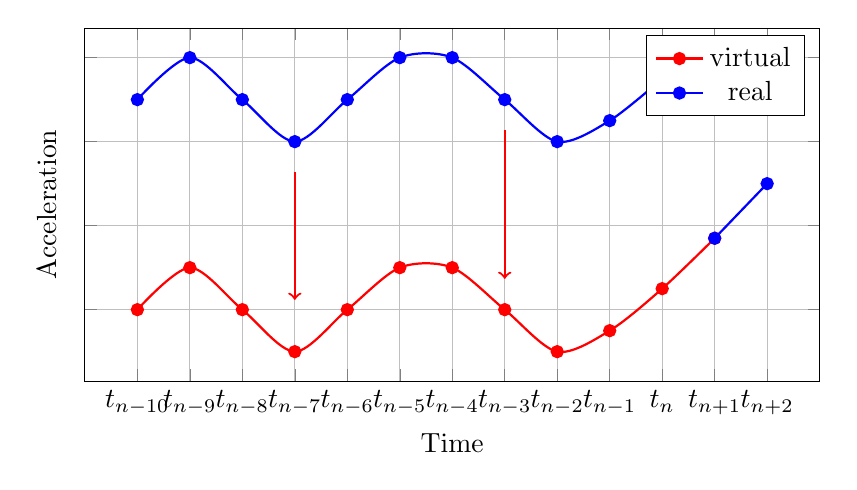
\begin{tikzpicture}[scale=1]

  \begin{axis}[
      height=0.5\textwidth,
      width=0.9\textwidth,
      xlabel = {Time},
      ylabel = {Acceleration},
      /pgf/number format/precision=10,
      xmin   = 0,
      xmax   = 14,
      %clip=false,
      %restrict x to domain=23:25,
      %x coord trafo/.code={\pgfmathparse{#1-5.0}\pgfmathresult} % x-offset MJD
      %ymin   = 0,
      %ymax   = 0.01,
      xtick  = {1,2,3,4,5,6,7,8,9,10,11,12,13,14},
      %ytick  = {},
      %minor x tick num={1},
      %minor y tick num={3},
      scaled ticks = true,
      ymajorgrids,
      yminorgrids,
      xmajorgrids,
      xminorgrids,
      yticklabels={,,},
      xticklabels={$t_{n-10}$,$t_{n-9}$,$t_{n-8}$,$t_{n-7}$,$t_{n-6}$,$t_{n-5}$,$t_{n-4}$,$t_{n-3}$,$t_{n-2}$,$t_{n-1}$,$t_{n}$,$t_{n+1}$,$t_{n+2}$},
      legend entries={virtual, real} ,
      %legend style={at={(0.02,0.98)}, anchor=north west},
      %legend cell align = left
      %every y tick label/.append style  =
       % { 
        %  /pgf/number format/.cd,
         %  precision = 3, 
          % fixed
        %}
  ]
    
    \addplot[red,thick,mark=*,smooth]  coordinates {(1,15-5)(2,16-5)(3,15-5)(4,14-5)(5,15-5)(6,16-5)(7,16-5)(8,15-5)(9,14-5)(10,14.5-5)(11,15.5-5)(12,16.7-5)};
    
    \addplot[blue,thick,mark=*,smooth]  coordinates {(1,15)(2,16)(3,15)(4,14)(5,15)(6,16)(7,16)(8,15)(9,14)(10,14.5)(11,15.5)
    
                                                     (12,16.7-5)(13,18-5)};
                                                     
    \node (source1)      at   ( axis cs: 4,13.5 ){};
    \node (destination1) at   ( axis cs: 4,10   ){};
    
    \node (source2)      at   ( axis cs: 8,14.5 ){};
    \node (destination2) at   ( axis cs: 8,10.5 ){};
    
    \draw[->,thick,red](source1)--(destination1);
    \draw[->,thick,red](source2)--(destination2);
    
    %\node (c1) at (axis cs:2,0.224309) {$\cdot 10^{-3}$};
  \end{axis}
  
\end{tikzpicture}
\caption{Method of modified back differences (\cite{lundberg1991})  \label{ax:accmod}}
\end{figure}
 These modified accelerations are only virtual but enable a continuous integration without any need of reinitialization due to the artificial smoothing effect. Consequently, the orbit propagation continues with the modified set of accelerations as if no shadow boundaries were crossed but with the correct acceleration conditions at the predicted state vector. The ``Lundberg-Correction'' is subdivided into two procedures:
 \begin{enumerate}
  \item Correction of the predicted state vector,
  \item Modification of the calculated back differences.
 \end{enumerate}
By crossing shadow boundaries, the predicted state vector is in error due to the additional accelerations implied by the crossing itself. Since the previous state vector sees a different \gls{acr:srp} acceleration as the predicted state vector, the acceleration in between both states has to be considered in order to achieve maximum accuracy. Due to the implied shadow function (see \cha{sec:propagation-state-srp-shadow}), the correction made to the predicted state vector can be formulated to
\begin{equation}
 \delta \gls{sym:radvec}_{\gls{idx:predict}} = \left[\frac{1}{2}\left(\gls{sym:t}_{\gls{sym:n}-\gls{sym:t}_{\gls{idx:c2}}}\right)^{2}+\frac{1}{6}\left(\gls{sym:t}_{\gls{idx:c2}}-\gls{sym:t}_{\gls{idx:c1}}\right)^{2}\right] \cdot \gls{sym:avec}_{\gls{sym:srp}}
 \label{equ:statecorrection}
\end{equation}
whereas the correction to the velocity term is calculated to
\begin{equation}
 \delta \gls{sym:radvecdot}_{\gls{idx:predict}} = \left[\left(\gls{sym:t}_{\gls{sym:n}-\gls{sym:t}_{\gls{idx:c2}}}\right)+\frac{1}{2}\left(\gls{sym:t}_{\gls{idx:c2}}-\gls{sym:t}_{\gls{idx:c1}}\right)\right] \cdot \gls{sym:avec}_{\gls{sym:srp}}.
 \label{equ:velocitycorrection}
\end{equation}
Therein, $\gls{sym:t}_{\gls{idx:c1}}$ and $\gls{sym:t}_{\gls{idx:c2}}$ are the first and second crossing times where the shadow condition changes. This issue is addressed more
detailed in \cha{sec:propagation-state-srp-shadow}. The differences \eq{equ:statecorrection} and \eq{equ:velocitycorrection} are being subtracted from the calculated state vector,
if the shadow is entered, and vice versa. To incorporate the modified accelerations into the predictor and corrector formula, the acceleration differences
$\gls{sym:phi_acc}_{\gls{idx:i}}$ (\eq{equ:dividedbackdifferences1} and \eq{equ:dividedbackdifferences2}) are modified with
\begin{equation}
 \gls{sym:phi_acc}_{\gls{idx:i}} = \gls{sym:phi_acc}_{\gls{idx:i}} - \delta \gls{sym:avec}_{\gls{sym:srp},\gls{idx:i}}
\end{equation}
to match the previous acceleration values with the conditions after crossing the shadow boundary. From there, the integrator continues as before using \eq{equ:predictor} and \eq{equ:corrector} without having to restart the initialization process respectively without any kind of delay due to the acceleration discontinuity. 

%------------------------------------------------------------------------------
\subsubsection{Considering orbital maneuvers}
\label{sec:propagation-state-maneuvers}
%------------------------------------------------------------------------------

Similar to acceleration discontinuities caused by shadow boundary crossings, as described in the previous section, impulsive orbital manoeuvres would also tend to induce an
integrator restart. In a research study by \citet{weidemeyer2013} the Lundberg algorithm was adapted to account for manoeuvres. The results, however, suggested that the
benefit of using this method versus simply re-starting the integrator is only marginal considering the low rate of manoeuvres for typical satellites. The design choice for
\neptune therefore was to use the Lundberg algorithm only for shadow boundary crossings (\sect{sec:propagation-state-integration-shadow}) and allow for re-starts of the integrator
in case of other acceleration discontinuities.

It is possible to provide a list of manoeuvres to be accounted for by \neptune during the propagation time span. For a flexible implementation, manoeuvres may be specified by an 
arbitrary number of phases with constant thrust, which basically allows to model any thrust curve. An example showing the syntax for different manoeuvres with varying number of
phases is shown in \lis{lis:manoeuvre-specification}.
\begin{listing}[H]
\begin{small}
\begin{minted}[bgcolor=mintedbg]{text}
      #         Date           Duration    a_u   a_v   a_w     
      #__[YYYY-MM-DDThh:mm:ss]____[s]______[*]___[*]___[*]___
          2009-04-20T18:03:00     70.0     20.0 -20.0   0.0    
                                  40.0     15.0 -20.0   0.0    
          2009-05-01T12:05:00     40.0      0.0  10.0   0.0    
                                  20.0      0.0  20.0   0.0    
                                  15.0      0.0  10.0   0.0    
          2009-05-01T12:10:00    100.0     40.0   0.0   0.0    
                                 200.0     30.0   0.0   0.0    
                                  20.0     50.0   0.0   0.0    
                                  20.0     30.0   0.0   0.0    
          2009-05-02T21:00:00     20.0      0.0 300.0   0.0 
\end{minted}
\caption{Specifying manoeuvres in \neptune to be considered during the propagation time span. \label{lis:manoeuvre-specification}}
\end{small}
\end{listing}
A single manoeuvre phase is provided as a constant acceleration of fixed duration in radial ($U$), along-track ($V$) and cross-track ($W$) components. The manoeuvre specification
is then converted into an acceleration curve as shown in \fig{fig:manoeuvre-model}.
\begin{figure}[h!]
 \centering
 \begin{tikzpicture}[>= latex]
 
  % Coordinates
  \draw[->] (-0.1,0) -- (8.5,0);
  \draw[->] (0,-0.1) -- node[left, very near end] {$\gls{sym:avec}\left(\gls{sym:t}\right)$} (0,4.5);
  
  % Maneuvers
  \draw[gray80, dashed] (0.5,1) -- (8,1);
  \draw[ilr-blue, thick] (2,2) -- (4,2) node[text=black, midway, anchor=south] {$\gls{sym:manoeuvre}_{1,p1}$};
  \draw[ilr-blue, thick] (5,4) -- (6,4) node[text=black, midway, anchor=south] {$\gls{sym:manoeuvre}_{1,p2}$};
  
  % Dotted lines
  \draw[gray50, dotted] (1,1) -- (1,-0.1) node[black, anchor=north] {$t_0$};
  \draw[gray50, dotted] (2,2) -- (2,-0.1) node[black, anchor=north] {$t_1$};
  \draw[gray50, dotted] (4,2) -- (4,-0.1) node[black, anchor=north] {$t_2$};
  \draw[gray50, dotted] (5,4) -- (5,-0.1) node[black, anchor=north] {$t_3$};
  \draw[gray50, dotted] (6,4) -- (6,-0.1) node[black, anchor=north] {$t_4$};
  \draw[gray50, dotted] (7,1) -- (7,-0.1) node[black, anchor=north] {$t_5$};
  
  % Transition t0 -> t1
  \draw[xshift=1cm, domain=0:1,smooth,variable=\x, thick, ilr-blue] plot ({\x},{(2.0*\x*\x*\x-3.0*\x*\x+1.0)+2.0*(3.0*\x*\x-2.0*\x*\x*\x)});
  
  % Transition t2 -> t3
  \draw[xshift=4cm, domain=0:1,smooth,variable=\x, thick, ilr-blue] plot ({\x},{2.0*(2.0*\x*\x*\x-3.0*\x*\x+1.0)+4.0*(3.0*\x*\x-2.0*\x*\x*\x)});
  
  % Transition t4 -> t5
  \draw[xshift=6cm, domain=0:1,smooth,variable=\x, thick, ilr-blue] plot ({\x},{4.0*(2.0*\x*\x*\x-3.0*\x*\x+1.0)+(3.0*\x*\x-2.0*\x*\x*\x)});
  
  % Nodes
  \node[] at (1.3,1.7) {$\gls{sym:transition}_{\gls{idx:start}}$};
  \node[] at (4.2,3.0) {$\gls{sym:transition}_{\gls{idx:phase}}$};
  \node[] at (6.7,3.0) {$\gls{sym:transition}_{\gls{idx:end}}$};
  
  % Info text
  \draw[xshift=7.5cm, yshift=3cm] node[right, text width=6cm, information text]{%
  \begin{tabular}{ll}
   $\gls{sym:manoeuvre}_{1,p1}$ & Manoeuvre 1, phase 1 \\
   $\gls{sym:manoeuvre}_{1,p2}$ & Manoeuvre 1, phase 2 \\
   $\gls{sym:transition}_{\gls{idx:start}}$ & Transition at start \\
   $\gls{sym:transition}_{\gls{idx:phase}}$ & Transition between phases  \\
   $\gls{sym:transition}_{\gls{idx:end}}$ & Transition at end \\
  \end{tabular}

  };
  
 \end{tikzpicture}
 \caption{Model to consider manoeuvres in \neptune, including multiple manoeuvre phases and phase transitions with cubic Hermite interpolation.\label{fig:manoeuvre-model}}
\end{figure}
The different thrust levels of subsequent manoeuvre phases are connected by short transition periods using cubic Hermite splines:
\begin{equation}
 \gls{sym:hermite}\left(\gls{sym:t}\right) = \left(2\gls{sym:t}^3-3\gls{sym:t}^2+1\right)\gls{sym:hermite}_0+\left(-2\gls{sym:t}^3+3\gls{sym:t}^2\right)\gls{sym:hermite}_1, \;
\gls{sym:t} \in \left[0,1\right] \label{eq:hermite-spline}
\end{equation}
here $\gls{sym:hermite}_0$ is the acceleration at the begin and $\gls{sym:hermite}_1$ at the end of the transition phase, respectively. Note that the above formulation in
\eq{eq:hermite-spline} deviates from the general formulation for cubic Hermite splines, because it is assumed that the tangent of the polynomial at the two end points is zero. 
As the spline is only valid for $\gls{sym:t} \in \left[0,1\right]$, the time coordinate of the integrator $\gls{sym:t}_{\gls{idx:int}}$ has to be converted, exemplarily for the
transition at manoeuvre start, according to:
\begin{equation}
 \gls{sym:t} = \frac{\gls{sym:t}_{\gls{idx:int}} - \gls{sym:t}_0}{\gls{sym:t}_1-\gls{sym:t}_0}
\end{equation}

The advantage of introducing transition phases lies in avoiding discontinuities. However, the integrator will most probably still evaluate the acceleration during a manoeuvre
phase, due to the relatively long duration of those phases compared to only \SI{10}{\second} as the assumed transition period. Typically that step will most likely fail, so that
the integrator will reduce the step size consequently and, hopefully, evaluate during the smooth transition, where the increase in acceleration might be accepted within the error
tolerance. Some experiments showed exactly this behaviour, while others did not. So, using transition phases in a variable step integrator might be thought of being non-essential
overhead. However, the implementation is quite easy and the additional evaluation cost is negligible.

Another problem is that, for short manoeuvres, the integrator might even miss the manoeuvre at all by evaluating before the manoeuvre and the subsequent step after the manoeuvre.
Therefore, it is necessary to implement a method which adapts the stepsize accordingly, so that manoeuvres will always be evaluated. In the current \neptune version, this is not
implemented yet.\todo[Manoeuvre issue]{It may happen that the integrator misses short manoeuvres for too high step sizes. The integrator (or the step size control) would have to
be adapted to account for this.}

%------------------------------------------------------------------------------
\subsection{Geopotential}
\label{sec:propagation-state-geopotential}
%------------------------------------------------------------------------------

The gravitational potential (or geopotential) provides the most important force for Earth-orbiting objects. Differentiating the potential for a point mass or a spherical body of
uniform density directly results in Newton's gravitational law. The general formulation for bodies of finite dimensions is more complicated. The derivation starts by integrating
potential contributions over all mass points in that body:
\begin{equation}
 \gls{sym:potential} = \gls{sym:gravConst} \int \frac{1}{\gls{sym:range}} d\gls{sym:mass},
\end{equation}
where the above integral contains the range between the orbiting mass point and each of the mass points of the central body. \citet{kaula2000} shows how to express the
potential in terms of spherical coordinates:
\begin{equation}
 \gls{sym:potential}\left(\gls{sym:r},\phigc,\gls{sym:long}\right) = \frac{\gls{sym:grav}}{\gls{sym:r}} 
     \sum\limits_{\gls{sym:geo_n}=2}^{\infty} \sum\limits_{\gls{sym:geo_m}=0}^{\gls{sym:geo_n}} 
      \left(\frac{\re}{\gls{sym:r}}\right)^{\gls{sym:geo_n}} \left(\cnm{}{} \cos \left(\gls{sym:geo_m}\gls{sym:long}\right) + 
\snm{}{} \sin \left(\gls{sym:geo_m}\gls{sym:long}\right)\right) \legphi{}{} \label{eq:geopotential}
\end{equation}
The potential is thus represented as an infinite sum of spherical harmonics with degree \gls{sym:geo_n} and order \gls{sym:geo_m} as a function of the radius
\gls{sym:r}, the geocentric latitude \phigc and the longitude \gls{sym:long}. Note that \eq{eq:geopotential} only contains the terms of the non-spherical part of the potential. 

The accelerations required for the orbit propagation are obtained by differentiating the potential with respect to the radius vector, the latter given in a body-fixed
frame:
\begin{equation}
 \gls{sym:avec}_{\gls{idx:bodyfixed}} = \frac{\partial \gls{sym:potential}}{\partial \rbf}
                = \frac{\partial \gls{sym:potential}}{\partial \gls{sym:r}} \left(\frac{\partial \gls{sym:r}}{\partial \rbf}\right)^T
                + \frac{\partial \gls{sym:potential}}{\partial \phigc} \left(\frac{\partial \phigc}{\partial \rbf}\right)^T
                + \frac{\partial \gls{sym:potential}}{\partial \gls{sym:long}} \left(\frac{\partial \gls{sym:long}}{\partial \rbf}\right)^T \label{eq:geopotential-acc-bf}
\end{equation}
The result obtained from \eq{eq:geopotential-acc-bf} is the inertial acceleration of the satellite expressed in an Earth-fixed frame (e.g. \gls{acr:itrf}), so that only
the transformation to an inertial reference frame is required \citep{long1989}, or, more specifically in the context of \neptune, using the \gls{acr:gcrf} and the
\gls{acr:itrf}:
\begin{equation}
 \gls{sym:avec}_{\acrshort{acr:gcrf}} = \kot{gcrf}{itrf} \gls{sym:avec}_{\acrshort{acr:itrf}} \label{eq:ns-trafo}
\end{equation}

The evaluation of \eq{eq:geopotential-acc-bf} requires knowing the partial derivatives. In the next two sections, a detailed description of how to obtain them is given.
It also includes second derivatives of the Legendre functions, which will be required later on for the propagation of the covariance matrix.

\subsubsection{Associated Legendre functions}

The associated Legendre functions for positive and integer $\gls{sym:geo_n}$ and $\gls{sym:geo_m}$ are typically given
in literature by a formulation including 
the derivatives of the ordinary Legendre functions:
\begin{equation}
 \gls{sym:legendre}_{\gls{sym:geo_n}}^{\gls{sym:geo_m}}\left(\gls{sym:xg}\right) = \left(-1\right)^{\gls{sym:geo_m}} 
\left(1-\gls{sym:xg}^2\right)^{\gls{sym:geo_m}/2} \frac{d^{\gls{sym:geo_m}}}{d\gls{sym:xg}^{\gls{sym:geo_m}}} 
\gls{sym:legendre}_{\gls{sym:geo_n}}\left(\gls{sym:xg}\right) \label{eq:legendre-function}
\end{equation}
Using the Rodrigues formula \citep{rodrigues1816} for ordinary Legendre functions
\begin{equation}
\gls{sym:legendre}_{\gls{sym:geo_n}}\left(\gls{sym:xg}\right) = 
\frac{1}{2^{\gls{sym:geo_n}}\gls{sym:geo_n}!}\frac{d^{\gls{sym:geo_n}}}{d\gls{sym:xg}^{\gls{sym:geo_n}}} \left(\gls{sym:xg}^2-1\right)^{\gls{sym:geo_n}},
\end{equation}
the associated Legendre functions can be expressed in the following form:
\begin{equation}
 \gls{sym:legendre}_{\gls{sym:geo_n}}^{\gls{sym:geo_m}}\left(\gls{sym:xg}\right) = 
\frac{\left(-1\right)^{\gls{sym:geo_m}}}{2^{\gls{sym:geo_n}}\gls{sym:geo_n}!} 
\left(1-\x^2\right)^{\gls{sym:geo_m}/2} \frac{d^{\gls{sym:geo_n}+\gls{sym:geo_m}}}{d\gls{sym:xg}^{\gls{sym:geo_n}+\gls{sym:geo_m}}} 
\left(\x^2-1\right)^{\gls{sym:geo_n}}. \label{eq:definition-legendre}
\end{equation}
Now it is important to note that the term $\left(-1\right)^{\gls{sym:geo_m}}$, known as the Condon-Shortley phase
in quantum mechanics, is typically not used for spherical harmonics as applied in geodesy or orbital mechanics. Thus,
various authors provide the definition of associated Legendre polynomials without the Condon-Shortley phase, e.g.
\cite{vallado2013}. This has to be considered, for example, when working with recurrence relations and derivatives later
on, especially when they are taken or derived from the work of different authors. In order to distinguish formulations
with and without Condon-Shortley phase, 
\cite{abramowitz1964} introduce a different notation:
\begin{equation}
 %\gls{sym:legendre}_{\gls{sym:geo_n}\gls{sym:geo_m}} 
\leg{}{} = \left(-1\right)^{\gls{sym:geo_m}} \gls{sym:legendre}_{\gls{sym:geo_n}}^{\gls{sym:geo_m}} \left(\gls{sym:xg}\right) \label{eq:condon-shortley}
\end{equation}
Thus, in the following, lower subscripts for both, degree \gls{sym:geo_n} and order \gls{sym:geo_m}, will correspond to
associated Legendre polynomials without 
the Condon-Shortley phase.

The derivative of the associated Legendre function with respect to the independent variable $\gls{sym:xg}$ can be
obtained by simply differentiating 
\eq{eq:definition-legendre}, taking into account the convention \eq{eq:condon-shortley}:
\begin{eqnarray}
 % Derivatives of Legendre Functions
\frac{d\leg{}{}}{d\x} &=& \frac{1}{2^{\gls{sym:geo_n}}\gls{sym:geo_n}!} \left( \frac{d}{d\x}\left[\left(1-\x^2\right)^{\gls{sym:geo_m}/2}\right] 
\frac{d^{\gls{sym:geo_n}+\gls{sym:geo_m}}}{d\x^{\gls{sym:geo_n}+\gls{sym:geo_m}}} 
\left(\x^2-1\right)^{\gls{sym:geo_n}}\right. + \nonumber\\
 & &\left.+\left(1-\x^2\right)^{\gls{sym:geo_m}/2} \frac{d}{d\x}\left[\frac{d^{\gls{sym:geo_n}+\gls{sym:geo_m}}}{d\x^{\gls{sym:geo_n}+\gls{sym:geo_m}}} 
\left(\x^2-1\right)^{\gls{sym:geo_n}}\right]\right) \nonumber \\
 &=& \frac{1}{2^{\gls{sym:geo_n}}\gls{sym:geo_n}!} 
\left(-\gls{sym:geo_m}\frac{\x}{1-\x^2}\left(1-\x^2\right)^{\gls{sym:geo_m}/2}\frac{d^{\gls{sym:geo_n}+\gls{sym:geo_m}}}{d\x^{\gls{sym:geo_n}+\gls{sym:geo_m}}} 
\left(\x^2-1\right)^{\gls{sym:geo_n}}\right. + \nonumber \\
 & &\left. +\frac{\left(1-\x^2\right)^{\frac{\gls{sym:geo_m}+1}{2}}}{\sqrt{1-\x^2}} 
\frac{d^{\gls{sym:geo_n}+\gls{sym:geo_m}+1}}{d\x^{\gls{sym:geo_n}+\gls{sym:geo_m}+1}} 
\left(\x^2-1\right)^{\gls{sym:geo_n}}\right) \nonumber \\
 \frac{d\leg{}{}}{d\x} &=& -\gls{sym:geo_m}\frac{\x}{1-\x^2} \leg{}{} + \frac{1}{\sqrt{1-\x^2}}\leg{}{+1} \label{eq:legendre-derivative}
\end{eqnarray}
The second derivative is determined analogously (only final result shown):
\begin{equation}
\begin{aligned}
 \frac{d^2\leg{}{}}{d\x^2} = &\frac{1}{\left(1-\x^2\right)^2} 
\left(\gls{sym:geo_m}^2-\gls{sym:geo_m}\x^2-\left(1-\x^2\right)\gls{sym:geo_n}\left(\gls{sym:geo_n}+1\right)\right) \leg{}{} + \\
 &+\frac{\x}{\left(1-\x^2\right)^{3/2}} \leg{}{+1} \label{eq:legendre-derivative-2}
\end{aligned}
\end{equation}
As the derivatives will be required with respect to the geocentric latitude, \phigc, and the independent variable of
the Legendre polynomials will be the $\sin 
\phigc$, a transformation is required:
\begin{eqnarray}
 \x  &=& \sin \left(\phigc\right) \nonumber \\
 \mathrm{d}\x &=& \cos \left(\phigc\right) \mathrm{d}\phigc \nonumber
\end{eqnarray}
Putting this into \eq{eq:legendre-derivative} and \eq{eq:legendre-derivative-2} one obtains:
\begin{eqnarray}
 \frac{\mathrm{d}\leg{}{}}{\mathrm{d}\phigc} &=& -\gls{sym:geo_m}\tan \phigc \legphi{}{} + \legphi{}{+1} \label{eq:deriv-legendre-phi}\\
 \frac{\mathrm{d}^2\leg{}{}}{\mathrm{d}\phigc^2} &=& \left(\gls{sym:geo_m}\sec^2 
\phigc-\gls{sym:geo_m}\tan^2\phigc-\gls{sym:geo_n}\left(\gls{sym:geo_n}+1\right)\right)\legphi{}{} + \nonumber\\
 & &+ \tan\phigc\legphi{}{+1} \label{eq:deriv-legendre-phi-2}
\end{eqnarray}

\subsubsection{Recursive formulation for computing the Legendre functions}

In the formulation of the geopotential in \eq{eq:geopotential}, the associated Legendre functions need to be evaluated. The latter can be computed using
\eq{eq:legendre-function}, but this is a laborious task, even for computers. A much easier way to obtain the results for given degree and order, is to use recursions.
According to \citet{montenbruck2000}, again using the relation $x = \sin\phigc$:
\begin{align}
 \gls{sym:legendre}_{\gls{sym:geo_m},\gls{sym:geo_m}} \left(\gls{sym:xg}\right) &= 
      \left(2\gls{sym:geo_m}-1\right)\sqrt{1-\gls{sym:xg}^2}\gls{sym:legendre}_{\gls{sym:geo_m}-1,\gls{sym:geo_m}-1} \label{eq:recurrence-legendre-1}\\
 \gls{sym:legendre}_{\gls{sym:geo_m}+1,\gls{sym:geo_m}} \left(\gls{sym:xg}\right) &=
      \left(2\gls{sym:geo_m}+1\right)\gls{sym:xg}\gls{sym:legendre}_{\gls{sym:geo_m},\gls{sym:geo_m}} \left(\gls{sym:xg}\right) \label{eq:recurrence-legendre-2}\\
 \leg{}{} &=
\frac{1}{\gls{sym:geo_n}-\gls{sym:geo_m}}\left(\left(2\gls{sym:geo_n}-1\right)\gls{sym:xg}\leg{-1}{}-\left(\gls{sym:geo_n}+\gls{sym:geo_m}-1\right)\leg{-2}{}\right), \;
 \forall \gls{sym:geo_n}>\gls{sym:geo_m}+1 \label{eq:recurrence-legendre-3},
%\frac{1}{\gls{sym:geo_n}}\left(\left(2\gls{sym:geo_n}-1\right)\gls{sym:xg}\gls{sym:legendre}_{\gls{sym:geo_n}-1,0}\left(\gls{sym:xg}\right)-\left(\gls{sym:geo_n}-1\right)
% \gls{sym:legendre}_{\gls{sym:geo_n},0} \left(\gls{sym:xg}\right) &=
%\frac{1}{\gls{sym:geo_n}}\left(\left(2\gls{sym:geo_n}-1\right)\gls{sym:xg}\gls{sym:legendre}_{\gls{sym:geo_n}-1,0}\left(\gls{sym:xg}\right)-\left(\gls{sym:geo_n}-1\right)
%\gls{sym:legendre}_{\gls{sym:geo_n}-2,0}\left(\gls{sym:xg}\right) \right), \; \gls{sym:geo_n} \geq 2 \label{eq:recurrence-legendre-1} \\
% \leg{}{} &= \leg{-2}{} + \left(2\gls{sym:geo_n}-1\right)\sqrt{1-\gls{sym:xg}^2}\leg{-1}{-1}, \; \gls{sym:geo_m} \neq 0, \gls{sym:geo_m}<\gls{sym:geo_n}
%\label{eq:recurrence-legendre-2}\\
% \gls{sym:legendre}_{\gls{sym:geo_n},\gls{sym:geo_n}} \left(\gls{sym:xg}\right) &= \left(2\gls{sym:geo_n}-1\right)\sqrt{1-\gls{sym:xg}^2}
%\gls{sym:legendre}_{\gls{sym:geo_n}-1,\gls{sym:geo_n}-1} \left(\gls{sym:xg}\right), \; \gls{sym:geo_n} \neq 0 \label{eq:recurrence-legendre-3}
\end{align}
with starting values being
\begin{align}
 \gls{sym:legendre}_{0,0}\left(\gls{sym:xg}\right) &= 1 \\
 \gls{sym:legendre}_{1,0}\left(\gls{sym:xg}\right) &= \gls{sym:xg} = \sin\phigc \\
 \gls{sym:legendre}_{1,1}\left(\gls{sym:xg}\right) &= \sqrt{1-\gls{sym:xg}^2} = \cos\phigc.
\end{align}

An important point, especially related to computation, is the fact that a recurrence formulation may become instable after the evaluation of a certain terms. This
means that through the loss of precision, the results become useless. This happens, for example, if differences of two nearly equal numbers are processed, or if there
are small divisors \citep{vallado2013}. In order to have a stable recurrence for the Legendre polynomials, a scheme as shown in \fig{fig:legendre-evaluation} has to be
followed with \eq{eq:recurrence-legendre-1} through \eq{eq:recurrence-legendre-3} \citep{montenbruck2000, brumberg1995}.
\begin{figure}[h!]
 \centering
   \begin{tikzpicture}[>=latex, every node/.style={inner sep=0.3cm}, node distance=0.5cm]
   
   \node (p00) {$\gls{sym:legendre}_{0,0}$};
   \node[below=of p00] (p10) {$\gls{sym:legendre}_{1,0}$};
   \node[below=of p10] (p20) {$\gls{sym:legendre}_{2,0}$};
   \node[below=of p20] (pd0) {$\vdots$};
   \node[below=of pd0] (pn0) {$\gls{sym:legendre}_{n,0}$};
   
   \draw[->] (p00) -- (p10);
   \draw[->] (p10) -- (p20);
   \draw[->] (p20) -- (pd0);
   \draw[->] (pd0) -- (pn0);
   
   \node[right=of p10] (p11) {$\gls{sym:legendre}_{1,1}$};
   \node[below=of p11] (p21) {$\gls{sym:legendre}_{2,1}$};
   \node[below=of p21] (pd1) {$\vdots$};
   \node[below=of pd1] (pn1) {$\gls{sym:legendre}_{n,1}$};
   
   \draw[->] (p00) -- (p11);
   \draw[->] (p11) -- (p21);
   \draw[->] (p21) -- (pd1);
   \draw[->] (pd1) -- (pn1);
   
   \node[right=of p21] (p22) {$\gls{sym:legendre}_{2,2}$};
   \node[below=of p22] (pd2) {$\vdots$};
   \node[below=of pd2] (pn2) {$\gls{sym:legendre}_{n,2}$};
   
   \draw[->] (p11) -- (p22);
   \draw[->] (p22) -- (pd2);
   \draw[->] (pd2) -- (pn2);
   
   \node[right=of pd2] (pd3) {$\ddots$};
   \node[below=of pd3] (pd4) {$\ldots$};
   
   \draw[->] (p22) -- (pd3);
   \draw[->] (pd3) -- (pd4);
      
   \node[right=of pd4] (pnn) {$\gls{sym:legendre}_{n,n}$};
   
   \draw[->] (pd3) -- (pnn);
   \draw[->] (pd4) -- (pnn);
   
   \matrix[right=3cm of p11](Mat){ 
			     \node (t1) {}; & \node {\eq{eq:recurrence-legendre-1}}; \\
			     \node (t2) {}; & \node (t4) {\eq{eq:recurrence-legendre-2}, \eq{eq:recurrence-legendre-3}};  \\ };
			   
   \draw[->] (t1.north west) -- (t1.south east);
   \draw[->] (t2.north) -- (t2.south);
   
   \begin{pgfonlayer}{background}
   \node[information text, fit= (t1) (t4)] {};
  \end{pgfonlayer}
   
\end{tikzpicture}
 \caption{Using a recurrence formulation for the Legendre functions.\label{fig:legendre-evaluation}}
\end{figure}
An interesting analysis on the stability of different recurrence formulations for the Legendre functions was done by \citet{lundberg1985}. The analysis showed that,
especially for high degree computations, the recurrence formulation in \eq{eq:recurrence-legendre-3} was superior to other formulations regarding stability. Just to show an
example, \fig{fig:legendre-unstable-example} gives the difference between the approach as described above, i.e. using \eq{eq:recurrence-legendre-1} through
\eq{eq:recurrence-legendre-3} in combination with the scheme shown in \fig{fig:legendre-evaluation}, and a different recurrence formulation (e.g. as given by \citet{long1989}),
without a specific scheme:
\begin{align}
\gls{sym:legendre}_{\gls{sym:geo_n},0} \left(\gls{sym:xg}\right) &=
\frac{1}{\gls{sym:geo_n}}\left(\left(2\gls{sym:geo_n}-1\right)\gls{sym:xg}\gls{sym:legendre}_{\gls{sym:geo_n}-1,0}\left(\gls{sym:xg}\right)-\left(\gls{sym:geo_n}-1\right)
 \gls{sym:legendre}_{\gls{sym:geo_n}-2,0}\left(\gls{sym:xg}\right) \right), \; \gls{sym:geo_n} \geq 2 \label{eq:recurrence-legendre-instable-1} \\
 \leg{}{} &= \leg{-2}{} + \left(2\gls{sym:geo_n}-1\right)\sqrt{1-\gls{sym:xg}^2}\leg{-1}{-1}, \; \gls{sym:geo_m} \neq 0, \gls{sym:geo_m}<\gls{sym:geo_n}
 \label{eq:recurrence-legendre-instable-2}\\
 \gls{sym:legendre}_{\gls{sym:geo_n},\gls{sym:geo_n}} \left(\gls{sym:xg}\right) &= \left(2\gls{sym:geo_n}-1\right)\sqrt{1-\gls{sym:xg}^2}
 \gls{sym:legendre}_{\gls{sym:geo_n}-1,\gls{sym:geo_n}-1} \left(\gls{sym:xg}\right), \; \gls{sym:geo_n} \neq 0 \label{eq:recurrence-legendre-instable-3}
\end{align}
\begin{figure}[h!]
 \centering
 \begin{tikzpicture} 
  \begin{axis}[
      y tick label style={
        /pgf/number format/.cd,
            fixed,
            fixed zerofill,
            precision=1,
        /tikz/.cd
       },
       xlabel = {Combined, geopotential degree and order $\left(n+\frac{m}{n+1}\right)$},
       ylabel = Error / \%,
       xmin=30,
       xmax=40,
       clip=false,
       xtick={30,31,...,40},
       grid=major,
       ytick scale label code/.code={$\cdot 10^{-7}$}
      ]
      
      \addplot[ilr-blue, thick] table {07-Tikz/data/legendre-unstable.temp2.dat};      
      %\node[fill=white, inner sep=0pt] (c1) at (axis cs:30.6,1.25e4) {$\cdot 10^{-7}$};
  \end{axis}
 \end{tikzpicture}
 \caption{Relative error between two different recurrence computation methods for the geopotential degree being between \num{30} and \num{40}. The first method
used \eq{eq:recurrence-legendre-1} through \eq{eq:recurrence-legendre-3} in combination with the scheme shown in \fig{fig:legendre-evaluation}, which is considered to be stable
according to \citet{montenbruck2000, brumberg1995, lundberg1985}. The second method uses the recurrence formulation given by \eq{eq:recurrence-legendre-instable-1} through
\eq{eq:recurrence-legendre-instable-3}. Both, the geopotential degree and order were combined as the independent variable $x$ according to
$x=\gls{sym:geo_n}+\frac{\gls{sym:geo_m}}{\gls{sym:geo_n}+1}$.\label{fig:legendre-unstable-example}}
\end{figure}

It can be seen in \fig{fig:legendre-unstable-example} that selecting a typical geopotential degree between \num{30} and \num{40} may already introduce significant errors, which
indicate that from \num{15} available digits only \num{7} or \num{8} actually contain useful information. The latter is especially true for those terms, where
$\gls{sym:geo_m}\approx \frac{\gls{sym:geo_n}}{2}$, while there is no difference between the two methods for zonal $\left(\gls{sym:geo_m}=0\right)$ or sectorial
$\left(\gls{sym:geo_n}=\gls{sym:geo_m}\right)$ terms. For higher degrees, the error grows exponentially.

\subsubsection{Other recurrence formulations}

Besides the Legendre functions, trigonometric terms may also be comfortably computed by using the following recursions:
\begin{align}
 \cos\gls{sym:geo_m} \gls{sym:long} &=
2\cos \left(\left(\gls{sym:geo_m}-1\right)\gls{sym:long}\right)\cos \gls{sym:long} - \cos\left(\left(\gls{sym:geo_m}-2\right)\gls{sym:long}\right) \\
\sin \gls{sym:geo_m} \gls{sym:long} &=
2\sin \left(\left(\gls{sym:geo_m}-1\right)\gls{sym:long}\right)\cos \gls{sym:long} - \sin\left(\left(\gls{sym:geo_m}-2\right)\gls{sym:long}\right)
\end{align}


\subsubsection{Derivatives of the disturbing potential function}

For the accelerations due to the geopotential, as given in \eq{eq:geopotential-acc-bf}, the derivatives with respect to the radius, the geocentric latitude and longitude are given
in the following:
\begin{equation}
 \label{eq:deriv-geopotential}
 \begin{aligned}
 %
 % Derivatives of potential function
 %
 % dU/dr
 \frac{\partial\gls{sym:potential}}{\partial\gls{sym:r}} =& -\frac{\gls{sym:grav}}{\gls{sym:r}^2} \sum\limits_{\gls{sym:geo_n}=2}^{\infty} 
\sum\limits_{\gls{sym:geo_m}=0}^{\gls{sym:geo_n}} \left(\frac{\re}{\gls{sym:r}}\right)^{\gls{sym:geo_n}} \left(\gls{sym:geo_n}+1\right) 
 \left(\cnm{}{} \cos \left(\gls{sym:geo_m}\gls{sym:long}\right) + \snm{}{} \sin \left(\gls{sym:geo_m}\gls{sym:long}\right)\right) \legphi{}{}  \\[1em]
 % dU/dphi
 \frac{\partial\gls{sym:potential}}{\partial\phigc} =& \frac{\gls{sym:grav}}{\gls{sym:r}} 
             \sum\limits_{\gls{sym:geo_n}=2}^{\infty} \sum\limits_{\gls{sym:geo_m}=0}^{\gls{sym:geo_n}} 
      \left(\frac{\re}{\gls{sym:r}}\right)^{\gls{sym:geo_n}} \left(\cnm{}{} \cos \left(\gls{sym:geo_m}\gls{sym:long}\right) + \snm{}{} \sin 
\left(\gls{sym:geo_m}\gls{sym:long}\right)\right) \times \\
 &\qquad \qquad \times \left(\legphi{}{+1} - \gls{sym:geo_m} \tan\phigc\legphi{}{} \right) \\[1em]
 % dU/dlambda
 \frac{\partial\gls{sym:potential}}{\partial\gls{sym:long}} =& \frac{\gls{sym:grav}}{\gls{sym:r}} 
     \sum\limits_{\gls{sym:geo_n}=2}^{\infty} \sum\limits_{\gls{sym:geo_m}=0}^{\gls{sym:geo_n}} 
      \left(\frac{\re}{\gls{sym:r}}\right)^{\gls{sym:geo_n}} \gls{sym:geo_m}\legphi{}{}\left(\snm{}{} \cos \left(\gls{sym:geo_m}\gls{sym:long}\right) - 
\cnm{}{} \sin \left(\gls{sym:geo_m}\gls{sym:long}\right)\right)
\end{aligned}
\end{equation}
It is interesting to note that although there is a $\tan\phigc$ term in the derivative with respect to the geocentric latitude, there is no singularity during 
evaluation of that function, as for the terms with $\gls{sym:geo_m}=0$ the term cancels and for $\gls{sym:geo_m}>0$ the Legendre polynomials $\legphi{}{}$ 
provide a $\cos\phigc$ term which reduces the tangent term to a sine term. 

The derivatives of the position vector in spherical coordinates \gls{sym:r}, {\phigc } and \gls{sym:long} with respect to the radius vector in the body-fixed frame 
are:
\begin{align}
 \frac{\partial\gls{sym:r}}{\partial\rbf} = & \frac{\rbf^T}{\gls{sym:r}} \label{eq:deriv-spherical-1} \\
 \frac{\partial\phigc}{\partial\rbf} = & \frac{1}{\sqrt{\gls{sym:r}_{\x}^2+\gls{sym:r}_{\y}^2}} 
\left(-\frac{\rbf^T\gls{sym:r}_{\gls{idx:z}}}{\gls{sym:r}^2}+\frac{\partial\gls{sym:r}_{\gls{idx:z}}}{\partial\rbf}\right) \\
 \frac{\partial\gls{sym:long}}{\partial\rbf} = & \frac{1}{\gls{sym:r}_{\x}^2+\gls{sym:r}_{\y}^2} 
\left(
\gls{sym:r}_{\gls{idx:x}}
\frac{\partial\gls{sym:r}_{\gls{idx:y}}}{\partial\rbf}-
\gls{sym:r}_{\gls{idx:y}}
\frac{\partial\gls{sym:r}_{\gls{idx:x}}}{\partial\rbf}
\right) \label{eq:deriv-spherical-3}
\end{align}

The resulting accelerations, including both, the central body terms, as well as the non-spherical part of the potential, are then obtained via:
\begin{eqnarray}
 % Geopotential inertial accelerations in body-fixed frame
 \gls{sym:a}_{\gls{idx:x},\gls{idx:bodyfixed}} &=& \left(\frac{1}{\gls{sym:r}}\frac{\partial \gls{sym:potential}}{\partial \gls{sym:r}}                          
                       -\frac{\gls{sym:r}_{\gls{idx:z}}}{\gls{sym:r}^2\sqrt{\gls{sym:r}^2_{\gls{idx:x}}+\gls{sym:r}^2_{\gls{idx:y}}}} \frac{\partial 
\gls{sym:potential}}{\partial \gls{sym:lat}_{\gls{idx:gc}}} \right) \gls{sym:r}_{\gls{idx:x}}
                                              -\left(\frac{1}{\gls{sym:r}^2_{\gls{idx:x}}+\gls{sym:r}^2_{\gls{idx:y}}} 
                                              \frac{\partial \gls{sym:potential}}{\partial \gls{sym:long}}\right) \gls{sym:r}_{\gls{idx:y}} -
\frac{\gls{sym:grav}\gls{sym:r}_{\gls{idx:x}}}{\gls{sym:r}^3}
\label{eq:geopotential-acceleration-1}\\
 \gls{sym:a}_{\gls{idx:y},\gls{idx:bodyfixed}} &=& \left(\frac{1}{\gls{sym:r}}\frac{\partial \gls{sym:potential}}{\partial \gls{sym:r}} 
                                       -\frac{\gls{sym:r}_{\gls{idx:z}}}{\gls{sym:r}^2\sqrt{\gls{sym:r}^2_{\gls{idx:x}}+\gls{sym:r}^2_{\gls{idx:y}}}} 
\frac{\partial \gls{sym:potential}}{\partial \gls{sym:lat}_{\gls{idx:gc}}} \right) \gls{sym:r}_{\gls{idx:y}}
                                              +\left(\frac{1}{\gls{sym:r}^2_{\gls{idx:x}}+\gls{sym:r}^2_{\gls{idx:y}}} \frac{\partial 
\gls{sym:potential}}{\partial \gls{sym:long}}\right) \gls{sym:r}_{\gls{idx:x}} \label{eq:geopotential-acceleration-2} -
\frac{\gls{sym:grav}\gls{sym:r}_{\gls{idx:y}}}{\gls{sym:r}^3} \\
 \gls{sym:a}_{\gls{idx:z},\gls{idx:bodyfixed}} &=& \frac{1}{\gls{sym:r}} \frac{\partial\gls{sym:potential}}{\partial\gls{sym:r}}\gls{sym:r}_{\gls{idx:z}} + 
\frac{\sqrt{\gls{sym:r}^2_{\gls{idx:x}}+\gls{sym:r}^2_{\gls{idx:y}}}}{\gls{sym:r}^2} \frac{\partial\gls{sym:potential}}{\partial\gls{sym:lat}} -
\frac{\gls{sym:grav}\gls{sym:r}_{\gls{idx:z}}}{\gls{sym:r}^3}
 \label{eq:geopotential-acceleration-3}
\end{eqnarray}

\subsubsection{Geopotential model providing harmonic coefficients}

The harmonic coefficients \cnm{}{} and \snm{}{} are obtained via observation. In the recent years, there have been a few missions providing new measurements of the geopotential
and thus an estimation of its harmonic coefficients: 
\begin{itemize}
 \item \gls{acr:champ}, \numrange{2000}{2010},
 \item \gls{acr:grace}, launched in March \num{2002}. 
 \item \gls{acr:goce}, \numrange{2009}{2013},
\end{itemize}
Follow-on missions are planned to further refine those estimates, e.g. \gls{acr:grace-fo}, which is a joint mission by \gls{acr:gfz} Potsdam and \gls{acr:nasa} planned for launch
in 2017\footnote{\url{http://gracefo.jpl.nasa.gov/mission/launchvehicle/}, accessed on February 9, 2015.}. It is important to note that besides the harmonic coefficients, \cnm{}{}
and \snm{}{}, also Earth's specific gravity constant $\gls{sym:grav}=\gls{sym:gravConst}\gls{sym:mbody}_{\gls{idx:earth}}$ and Earth's radius are estimated. Thus, it is important
that the following quantities are understood to be interrelated and therefore be used consistently:
\begin{itemize}
 \item Harmonic coefficients \cnm{}{} and \snm{}{},
 \item Earth's radius $\gls{sym:radius}_{\gls{idx:earth}}$ and
 \item Earth's specific gravity constant $\gls{sym:grav}=\gls{sym:gravConst}\gls{sym:mbody}_{\gls{idx:earth}}$.
\end{itemize}
All quantities are typically provided in a data file for a certain geopotential model. A very detailed list of past and current geopotential models is provided by the
\gls{acr:icgem} \footnote{\url{http://icgem.gfz-potsdam.de/ICGEM/}, accessed on February 9, 2015}. Incorporating data from ground measurements and satellite missions (as provided
above), today's models typically provide the geopotential up to degree and order of \num{2160}. In the space surveillance context, that level of detail is not required. The
individual models thus do not pose severe limitations with respect to selecting an adequate model for propagation in that context. Three different models were implemented in
\neptune{}:
\begin{itemize}
 \item \acrshort{acr:eigen}-GL04C (\acrlong{acr:eigen}),
 \item \acrshort{acr:egm}96 (\acrlong{acr:egm}) and
 \item \acrshort{acr:egm}2008.
\end{itemize}
It is simple to add an arbitrary new model to \neptune{}, as only an individual data file parser has to be provided. \neptune{} extracts the geopotential coefficients, associated
time derivatives (if available) and Earth's specific gravity constant as well as Earth's radius to be used in the propagation.

With harmonic coefficients being provided as normalized, it is important to de-normalize, before being combined with the Lagrange functions to compute the accelerations of the
geopotential. Alternatively, it is also possible to use normalized Legendre functions. However, the former approach was selected for \neptune{} with the following equation for the
de-normalization (normalized quantities provided with a bar):
\begin{equation}
 \left(\begin{array}{c}
        \overline{\gls{sym:geo_C}}_{\gls{sym:geo_n},\gls{sym:geo_m}} \\
        \overline{\gls{sym:geo_S}}_{\gls{sym:geo_n},\gls{sym:geo_m}} \\
       \end{array}
\right) = \sqrt{\frac{\left(\gls{sym:geo_n}+\gls{sym:geo_m}\right)!}{\gls{sym:deltam}\left(2\gls{sym:geo_n}+1\right)\left(\gls{sym:geo_n}-\gls{sym:geo_m}\right)!}}
\left(\begin{array}{c}
        \gls{sym:geo_C}_{\gls{sym:geo_n},\gls{sym:geo_m}} \\
        \gls{sym:geo_S}_{\gls{sym:geo_n},\gls{sym:geo_m}} \\
       \end{array}
\right), \label{eq:normalization}
\end{equation}
here
\begin{align}
 \gls{sym:deltam} &= 1, \; m=0, \notag \\
 \gls{sym:deltam} &= 2, \; m>0. \notag 
\end{align}


%------------------------------------------------------------------------------
%
\subsection{Gravitational perturbations due to solar system bodies}
\label{sec:propagation-state-3body}
%
%------------------------------------------------------------------------------

With \neptune being designed for objects orbiting the Earth, all other solar system bodies are contributing gravitational perturbations, which can be described by
Newton's gravitational law. The acceleration of a so-called third body can thus be expressed as:
\begin{equation}
 \gls{sym:avec}_{\gls{idx:3b}} =
\gls{sym:gravConst}\gls{sym:mbody}_{\gls{idx:3b}}\frac{\gls{sym:radvec}_{\gls{idx:3b}}-\gls{sym:radvec}_{\gls{idx:sat}}}{|\gls{sym:radvec}_{\gls{idx:3b}}-\gls{sym:radvec}
_{\gls{idx:sat}}|^3},
\end{equation}
with $\gls{sym:radvec}_{\gls{idx:3b}}$ and $\gls{sym:radvec}_{\gls{idx:sat}}$ being the geocentric radius vector of the third body and the satellite, respectively.

The contributions due to the Sun and the Moon are currently considered by \neptune. The geocentric coordinates as well as the mass are obtained via the \gls{acr:de}, the
latter being publicly available from the \gls{acr:jpl}.

\subsubsection{Using JPL ephemerides}

The \gls{acr:jpl} provides ephemerides for thousands of solar system bodies via its \textsc{Horizons} on-line system\footnote{\url{http://ssd.jpl.nasa.gov/?horizons},
accessed on February 11, 2015.}. However, in order to be independent of an internet connection to obtain the coordinates of the Moon and the Sun, those were pre-processed for \neptune{} and are available in two different \gls{acr:de} series:
\begin{itemize}
 \item DE 421, which was released in \num{2008}, contains latest measurements and covers the years from \numrange{1900}{2050} \citep{folkner2008}. This model is used by
\neptune as long as the propagation span is within that time interval.
 \item DE 405, which was released in \num{1998} covering a time interval from \numrange{1600}{2200} \citep{standish1998}.
\end{itemize}
The specific gravitational constant for both, Sun and Moon are used in accordance with the selected \gls{acr:de} series and are
given in \tab{tab:de-mu-sun-and-moon}.
\begin{table}[h!]
  \centering
  \caption{Specific gravity constant $\gls{sym:gravConst}\gls{sym:mbody}_{\gls{idx:3b}}$ for the Sun and the Moon as used in \neptune. \label{tab:de-mu-sun-and-moon}}
  \begin{tabular}{@{}lSS@{}}
   \toprule
   \multirow{2}{*}{Celestial body} & \multicolumn{2}{c}{Specific gravity constant $\gls{sym:gravConst}\gls{sym:mbody}_{\gls{idx:3b}}$ /
\si[per-mode=symbol]{\kilo\metre\cubed\per\second\squared}} \\
                                   & {DE 405} & {DE 421} \\
  \cmidrule{1-3}
   Sun  & 132712440017.987 & 132712440040.944 \\
   Moon & 4902.801 & 4902.800076 \\
   \bottomrule
  \end{tabular}

\end{table}

%------------------------------------------------------------------------------
%
\subsection{Solid Earth and ocean tides}
\label{sec:propagation-state-tides}
%
%------------------------------------------------------------------------------

Due to the gravitational forces of both, the Sun and the Moon, the figure of the Earth experiences time-varying, periodic deformations known as tides. There are two
contributions that are modeled independently:
\begin{itemize}
 \item \textit{Solid Earth tides} are referred to deformations of the solid figure of the Earth, while
 \item \textit{Ocean tides} result from the response of the Earth's oceans to luni-solar attraction.
\end{itemize}
The most convenient way of modeling tides is to induce variations in the geopotential coefficients \cnm{}{} and \snm{}{} \citep{luzum2010}. It is important, that the
geopotential model used is tide free, which is the case, for example, for the models used in \neptune: \acrshort{acr:eigen}-GL04C, \acrshort{acr:egm}96 and
\acrshort{acr:egm}2008. 

\subsubsection{Solid Earth tides}

To account for solid Earth tides, \citet{luzum2010} provides an equation for the correction of the normalized harmonic coefficients of the
geopotential:
\begin{equation}
 \left(\begin{array}{c}
        \Delta \overline{\gls{sym:geo_C}}_{\gls{sym:geo_n}\gls{sym:geo_m}} \\
        \Delta \overline{\gls{sym:geo_S}}_{\gls{sym:geo_n}\gls{sym:geo_m}}
       \end{array}
      \right)
      = \frac{\gls{sym:loveNumber}_{\gls{sym:geo_n}\gls{sym:geo_m}}}{2\gls{sym:geo_n}+1}
\left(\frac{\gls{sym:gravConst}\gls{sym:mbody}_{\gls{idx:3b}}}{\gls{sym:gravConst}\gls{sym:mbody}_{\gls{idx:earth}}}\right)\left(\frac{\gls{sym:radius}_{\gls{idx:earth}}}
{ \gls{sym:r}_{\gls{idx:3b}}}\right)^{\gls{sym:geo_n}+1}\overline{\gls{sym:legendre}}_{\gls{sym:geo_n}\gls{sym:geo_m}}\left(\sin\gls{sym:lat}_{\gls{idx:3b}}
\right)\left(\begin{array}{c}
              \cos\left(\gls{sym:geo_m}\gls{sym:long}_{\gls{idx:3b}}\right) \\
              \sin\left(\gls{sym:geo_m}\gls{sym:long}_{\gls{idx:3b}}\right)
             \end{array}
            \right)  \label{eq:solid-earth-tides}
\end{equation}
The above changes to the harmonic coefficients have to be applied for both, the Sun and the Moon, respectively. Besides the ephemerides and the mass, the geocentric
latitude and longitude of both, the Sun ($\gls{sym:lat}_{\gls{idx:sun}}, \gls{sym:long}_{\gls{idx:sun}}$) and the Moon ($\gls{sym:lat}_{\gls{idx:moon}},
\gls{sym:long}_{\gls{idx:moon}}$) is computed to be used in the normalized Legendre functions.

The $\gls{sym:loveNumber}_{\gls{sym:geo_n}\gls{sym:geo_m}}$ are the nominal Love numbers for degree \gls{sym:geo_n} and order \gls{sym:geo_m} of the \gls{acr:tgp}, as
given in \tab{tab:love-numbers}.
\begin{table}[h!]
 \centering
 \caption{Nominal values of solid Earth tide external potential Love numbers for the elastic Earth \citep{luzum2010}.\label{tab:love-numbers}}
 \begin{tabular}{ccSS}
  \toprule
  \gls{sym:geo_n} & \gls{sym:geo_m} & {$\gls{sym:loveNumber}_{\gls{sym:geo_n}\gls{sym:geo_m}}$} &
{$\gls{sym:loveNumber}^{\left(+\right)}_{\gls{sym:geo_n}\gls{sym:geo_m}}$} \\
  \midrule
  2 & 0 & 0.29525  & -0.00087 \\
  2 & 1 & 0.29470  & -0.00079 \\
  2 & 2 & 0.29801  & -0.00057 \\
  3 & 0 & 0.093    &   \\
  3 & 1 & 0.093    &   \\
  3 & 2 & 0.093    &   \\
  3 & 3 & 0.094    &   \\
  \bottomrule
 \end{tabular}
\end{table}

As \neptune is working with both, unnormalized coefficients as well as unnormalized Legendre functions, \eq{eq:solid-earth-tides} has to be converted, using the known
relationship between normalized and unnormalized quantities (see also \eq{eq:normalization}):
\begin{equation}
 \gls{sym:normalization}_{\gls{sym:geo_n}\gls{sym:geo_m}} =
\sqrt{\frac{\left(\gls{sym:geo_n}+\gls{sym:geo_m}\right)!}{\gls{sym:deltam}\left(2\gls{sym:geo_n}+1\right)\left(\gls{sym:geo_n}-\gls{sym:geo_m}\right)!}}
\end{equation}
with
\begin{equation}
 \left(\begin{array}{c}
        \overline{\gls{sym:geo_C}}_{\gls{sym:geo_n}\gls{sym:geo_m}} \\
        \overline{\gls{sym:geo_S}}_{\gls{sym:geo_n}\gls{sym:geo_m}}
       \end{array}
 \right) = \gls{sym:normalization}_{\gls{sym:geo_n}\gls{sym:geo_m}}
 \left(\begin{array}{c}
        \gls{sym:geo_C}_{\gls{sym:geo_n}\gls{sym:geo_m}} \\
        \gls{sym:geo_S}_{\gls{sym:geo_n}\gls{sym:geo_m}}
       \end{array}
 \right), \quad \text{and} \quad \overline{\gls{sym:legendre}}_{\gls{sym:geo_n}\gls{sym:geo_m}} =
\frac{\leg{}{}}{\gls{sym:normalization}_{\gls{sym:geo_n}\gls{sym:geo_m}}} \label{eq:normalization2}
\end{equation}
Substituting \eq{eq:normalization2} into \eq{eq:solid-earth-tides} one obtains the corrections to the unnormalized coefficients:
\begin{align}
 \left(\begin{array}{c}
        \Delta \cnm{}{} \\
        \Delta \snm{}{}
       \end{array}
      \right)
      &= \left(\begin{array}{c}
        \Delta \overline{\gls{sym:geo_C}}_{\gls{sym:geo_n}\gls{sym:geo_m}} \\
        \Delta \overline{\gls{sym:geo_S}}_{\gls{sym:geo_n}\gls{sym:geo_m}}
       \end{array}
      \right) \frac{1}{\gls{sym:normalization}_{\gls{sym:geo_n}\gls{sym:geo_m}}}
      = \frac{1}{\gls{sym:normalization}^2_{\gls{sym:geo_n}\gls{sym:geo_m}}} \frac{\gls{sym:loveNumber}_{\gls{sym:geo_n}\gls{sym:geo_m}}}{2\gls{sym:geo_n}+1}
\left(\frac{\gls{sym:gravConst}\gls{sym:mbody}_{\gls{idx:3b}}}{\gls{sym:gravConst}\gls{sym:mbody}_{\gls{idx:earth}}}\right)\left(\frac{\gls{sym:radius}_{\gls{idx:earth}}}
{ \gls{sym:r}_{\gls{idx:3b}}}\right)^{\gls{sym:geo_n}+1}\gls{sym:legendre}_{\gls{sym:geo_n}\gls{sym:geo_m}}\left(\sin\gls{sym:lat}_{\gls{idx:3b}}
\right)\left(\begin{array}{c}
        \cos\left(\gls{sym:geo_m}\gls{sym:long}_{\gls{idx:3b}}\right) \\
        \sin\left(\gls{sym:geo_m}\gls{sym:long}_{\gls{idx:3b}}\right)
       \end{array}
       \right) \notag \\
&= 
\gls{sym:loveNumber}_{\gls{sym:geo_n}\gls{sym:geo_m}}\gls{sym:deltam}\frac{\left(\gls{sym:geo_n}-\gls{sym:geo_m}\right)!}{\left(\gls{sym:geo_n}+\gls{sym:geo_m}\right)!}
\left(\frac{\gls{sym:gravConst}\gls{sym:mbody}_{\gls{idx:3b}}}{\gls{sym:gravConst}\gls{sym:mbody}_{\gls{idx:earth}}}\right)\left(\frac{\gls{sym:radius}_{\gls{idx:earth}}}
{ \gls{sym:r}_{\gls{idx:3b}}}\right)^{\gls{sym:geo_n}+1}\gls{sym:legendre}_{\gls{sym:geo_n}\gls{sym:geo_m}}\left(\sin\gls{sym:lat}_{\gls{idx:3b}}
\right)\left(\begin{array}{c}
              \cos\left(\gls{sym:geo_m}\gls{sym:long}_{\gls{idx:3b}}\right) \\
              \sin\left(\gls{sym:geo_m}\gls{sym:long}_{\gls{idx:3b}}\right)
             \end{array}\right)
\end{align}
Tides of degree \num{2} introduce changes in the geopotential coefficients of degree \num{4}, which also has to be considered. \citet{luzum2010} gives the corrections
for the normalized values. The result for unnormalized coefficients is obtained from \eq{eq:solid-earth-tides} using the transformation from \eq{eq:normalization}:
\begin{align}
  \left(\begin{array}{c}
        \Delta \gls{sym:geo_C}_{4\gls{sym:geo_m}} \\
        \Delta \gls{sym:geo_S}_{4\gls{sym:geo_m}}
       \end{array}
      \right)
       &=
\frac{1}{\gls{sym:normalization}_{4\gls{sym:geo_m}}\gls{sym:normalization}_{2\gls{sym:geo_m}}}
\frac{\gls{sym:loveNumber}^{\left(+\right)}_{\gls{sym:geo_n}\gls{sym:geo_m}}}{5}
\left(\frac{\gls{sym:gravConst}\gls{sym:mbody}_{\gls{idx:3b}}}{\gls{sym:gravConst}\gls{sym:mbody}_{\gls{idx:earth}}}
\right)\left(\frac{\gls{sym:radius}_{\gls{idx:earth}}}{\gls{sym:r}_{\gls{idx:3b}}}\right)^{3}\gls{sym:legendre}_{2\gls{sym:geo_m}} \left(\sin\gls{sym:lat}_{\gls{idx:3b}}
\right)\left(\begin{array}{c}
              \cos\left(\gls{sym:geo_m}\gls{sym:long}_{\gls{idx:3b}}\right) \\
              \sin\left(\gls{sym:geo_m}\gls{sym:long}_{\gls{idx:3b}}\right)
             \end{array}\right) \notag \\
&=\gls{sym:loveNumber}^{\left(+\right)}_{2\gls{sym:geo_m}}\gls{sym:deltam}\frac{\left(2-\gls{sym:geo_m}\right)!}{\left(2+\gls{sym:geo_m}\right)!}\sqrt{\frac{9\left(4-\gls
{sym:geo_m}\right)\left(3-\gls{sym:geo_m}\right)}{5\left(4+\gls{sym:geo_m}\right)\left(3+\gls{sym:geo_m}\right)}}\left(\frac{\gls{sym:gravConst}\gls{sym:mbody}_{
\gls{idx:3b}}}{\gls{sym:gravConst}\gls{sym:mbody}_{\gls{idx:earth}}}
\right)\left(\frac{\gls{sym:radius}_{\gls{idx:earth}}}{\gls{sym:r}_{\gls{idx:3b}}}\right)^{3}\gls{sym:legendre}_{2\gls{sym:geo_m}} \left(\sin\gls{sym:lat}_{\gls{idx:3b}}
\right)\left(\begin{array}{c}
              \cos\left(\gls{sym:geo_m}\gls{sym:long}_{\gls{idx:3b}}\right) \\
              \sin\left(\gls{sym:geo_m}\gls{sym:long}_{\gls{idx:3b}}\right)
             \end{array}\right),
\end{align}
with the above equation being used for $\gls{sym:geo_m}=0,1,2$ and the parameters $\gls{sym:loveNumber}^{\left(+\right)}_{2\gls{sym:geo_m}}$ given in
\tab{tab:love-numbers}.

Another correction is applied for the \textit{pole tide}, which is due to the centrifugal effect of polar motion \citep{luzum2010}. Again, the unnormalized corrections
are:
\begin{align}
  \Delta \gls{sym:geo_C}_{21} &= -1.721\cdot 10^{-9}\left(m_1-0.0115 m_2\right) \\
  \Delta \gls{sym:geo_S}_{21} &= -1.721\cdot 10^{-9}\left(m_2+0.0115 m_1\right)
\end{align}
The quantities $m_1$ and $m_2$ are defined as the deviations of the polar motion variables \gls{sym:pomx} and \gls{sym:pomy} from their running averages:
\begin{align}
 m_1 &= \gls{sym:pomx} - \overline{x}_p \\
 m_1 &= -\left(\gls{sym:pomy} - \overline{y}_p\right). \\
\end{align}
The running average is computed according to a time series given by \citet{luzum2010}:
\begin{equation}
 \left(\begin{array}{c}
  \overline{x}_p \left(t\right) \\
  \overline{y}_p \left(t\right)
 \end{array}\right) = \sum_{i=0}^{3} \left(t-t_0\right)^i \left(\begin{array}{c}
                                                                 \overline{x}_p^i \\
								 \overline{y}_p^i
                                                                \end{array}\right),
\end{equation}
with the coefficients given in \tab{tab:pole-tide-coeff} and $t_0$ corresponding to the epoch 2000.0.
\begin{table}[h!]
 \centering
 \caption{Coefficients of the IERS (2010) mean pole model \citep{luzum2010}.\label{tab:pole-tide-coeff}}
 \begin{tabular}{cSSSS}
  \toprule
  & \multicolumn{2}{c}{Until \num{2010.0}} & \multicolumn{2}{c}{After \num{2010.0}} \\
  \midrule
  Degree i & {$\overline{x}^i_p$ / mas yr$^{-i}$} & {$\overline{y}^i_p$ / mas yr$^{-i}$} & {$\overline{x}^i_p$ / mas yr$^{-i}$} & {$\overline{y}^i_p$ / mas yr$^{-i}$} \\
  \midrule
  0 & 55.974     & 346.346    & 23.513    &  358.891  \\
  1 & 1.8243     &  1.7896    &  7.6141   &   -0.6287 \\
  2 & 0.18413    & -0.10729   &  0.0      &    0.0    \\
  3 & 0.007024   & -0.000908  &  0.0      &    0.0    \\
  \bottomrule
 \end{tabular}\
 \end{table}

Due to the dependence on polar motion variables, the pole tide implementation is only considered in \neptune as long as \gls{acr:eop} are also considered. In
\fig{fig:tides-example}, an example is given for a \gls{acr:leo} satellite, showing the order of the position error introduced during propagation when omitting solid
Earth tides.

\subsubsection{Ocean tides}

The reaction of Earth's water mass to the gravitational forces of the Sun and the Moon is referred to as ocean tides, which provide a contribution of about
\SIrange{10}{15}{\percent} compared to solid Earth tides, as suggested by \citet{casotto1989}. Due to the very complex nature of the water motion, ocean tide models are typically
represented by models with a broad range of frequencies and amplitudes in the spectrum.

For \neptune, the current implementation is a simplified model of degree six as given by \citet{vallado2013}:
\begin{equation}
 \left(\begin{array}{c}
        \Delta \cnm{}{} \\
        \Delta \snm{}{} 
       \end{array}\right)
       =
\frac{4\gls{sym:pi}\gls{sym:radius}^2_{\gls{idx:earth}}\gls{sym:density}_{\gls{idx:water}}}{\gls{sym:mbody}_{\gls{idx:earth}}}\left(\frac{1+\gls{sym:loadDeformation}}{2
\gls{sym:geo_n}+1} \right) \left(\frac{\gls{sym:gravConst}\gls{sym:mbody}_{\gls{idx:3b}}}{\gls{sym:gravConst}\gls{sym:mbody}_{\gls{idx:earth}}}
\right)\left(\frac{\gls{sym:radius}_{\gls{idx:earth}}}{\gls{sym:r}_{\gls{idx:3b}}}\right)^{\gls{sym:geo_n}+1}\gls{sym:legendre}_{\gls{sym:geo_n}\gls{sym:geo_m}}\left(\sin
\gls{sym:lat}_{\gls{idx:3b}}\right)
\left(\begin{array}{c}
       \cos\left(\gls{sym:geo_m}\gls{sym:long}_{\gls{idx:3b}}\right) \\
       \sin\left(\gls{sym:geo_m}\gls{sym:long}_{\gls{idx:3b}}\right)
      \end{array}\right)
\end{equation}
with $\gls{sym:density}_{\gls{idx:water}}=\SI[per-mode=symbol]{1025}{\kilogram\per\metre\cubed}$ being the density of sea-water and \gls{sym:loadDeformation} being the load deformation
coefficients as given in \tab{tab:loadDeformation}.
\begin{table}[h!]
 \centering
 \caption{Load deformation coefficients according to \citet{luzum2010}.\label{tab:loadDeformation}}
 \begin{tabular}{cS}
  \toprule
  Degree \gls{sym:geo_n} & {\gls{sym:loadDeformation}} \\
  \midrule
  2 & -0.3075 \\
  3 & -0.195 \\
  4 & -0.132 \\
  5 & -0.1032 \\
  6 & -0.0892 \\
  \bottomrule
 \end{tabular}
\end{table}

For the next revision, an update of the ocean tides model is envisaged\todo[Ocean tide model update]{Update the Ocean tides model according to the IERS 2010 conventions} according
to the recommendation of the actual \gls{acr:iers} conventions \citep{luzum2010}. However, it is still possible to use a truncated model. For example, a truncation above degree six
was justified for \gls{acr:lageos} \citep{seidelmann2006}, being compliant with the requirement of determining the radial component in the cm-regime.

\citet{luzum2010} gives an example for the influence of ocean tides: For a satellite in an \SI{800}{\kilo\metre} orbit ($\gls{sym:inc}=\ang{98.7;;}$, $\gls{sym:ecc}=0.001$) and
one day of propagation, the error is on the order of several \si{\centi\metre} and reaches up to \SI{20}{\centi\metre}. For a similar satellite with that orbit, a simulation with
\neptune was performed, providing the expected result, as shown in \fig{fig:tides-example}

\begin{figure}[h!]
 \centering
 \begin{tikzpicture} 
  \begin{semilogyaxis}[
      %y tick label style={
      %  /pgf/number format/.cd,
      %      fixed,
      %      fixed zerofill,
      %      precision=1,
      %  /tikz/.cd
      % },
      x tick label style={
       /pgf/number format/.cd,
           fixed,
           fixed zerofill,
           precision=0,
       /tikz/.cd
      },
       scaled x ticks = false,
       xlabel = {Propagation time / days},
       ylabel = Position Error / km,
       xmin=0,
       xmax=7,
       %clip=false,
       xtick={0,1,2,3,4,5,6,7},
       grid=major,
       legend entries={Solid Earth tides, Ocean tides},
       legend style={at={(1.2,0.5)}, anchor=west, draw=none},
       legend cell align = left
      ]
      
      \addplot[dark-red, dashed, thick] table {07-Tikz/data/solidTideVs2body.red.out};  
      \addplot[ilr-blue, densely dotted, thick] table {07-Tikz/data/oceanTideVs2body.red.out};  
  \end{semilogyaxis}
 \end{tikzpicture}
 \caption{Solid Earth and ocean tides example for an \SI{800}{\kilo\metre} orbit ($\gls{sym:inc}=\ang{98.7;;}$, $\gls{sym:ecc}=0.001$). The position error is computed for a
trajectory comparison against a two-body propagation.\label{fig:tides-example}}
\end{figure}

%------------------------------------------------------------------------------
%
\subsection{Atmospheric drag}
\label{sec:propagation-state-drag}
%
%------------------------------------------------------------------------------
Using \eq{eq:drag-acceleration}, the atmospheric drag acceleration in the \gls{acr:gcrf} can be computed.
\begin{equation}
 \label{eq:drag-acceleration}
 \gls{sym:avec}_{\gls{idx:drag}} = 
-\frac{\density}{2} \cdot \frac{\cd \cdot \gls{sym:area}_{\gls{idx:cross}}}{\gls{sym:mass}} \cdot \relvel\left|\relvel\right|
\end{equation}
It is a function of the atmospheric density $\density$, the mass of the object $m$, its cross sectional area $A_c$ faced toward the direction of \relvel and the drag coefficient $c_D$. The atmospheric density is computed based on the \gls{acr:nrl} \gls{acr:msis} model, commonly known as NRLMSISE-00 atmopshere model. It takes as independent variables the desired
\begin{itemize}
\item date and time,
\item geographic altitude above NN,
\item geographic longitude and
\item geographic latitude.
\end{itemize}
Based on which it calculates the overall mass density in $g/cm^3$, as a result from the following parameters,
\begin{itemize}
\item Atomic Oxygen ($O$) count per volume,
\item Nitrogen ($N_2$) count per volume,
\item Oxygen ($O_2$) count per volume,
\item Helium ($He$) count per volume,
\item Argon ($Ar$) count per volume,
\item Hydrogen ($H$) count per volume,
\item Nitrogen ($N$) count per volume,
\item Anomalous Oxygen count per volume,
\item Neutral Temperature and
\item Exospheric Temperature.
\end{itemize}
As the density depends on external parameters, like the solar and geomagnetic activity the calculations prerequisite several indices:
\begin{itemize}
\item $F10.7$ (daily),
\item $F10.7$ (3-month average) and
\item $ap$ (daily),
\end{itemize}
where the $F10.7$ indicates the solar activity as the radiation with the wavelength of \SI{10.7}{\cm}, that correlates with the \gls{acr:euv} radiation. A \gls{acr:euv} influences the ionized layers of the atmosphere and thus results in a higher mass density. The geomagnetic $ap$ index in turn describes the particle radiation of the Sun and its interaction with the Earth's magnetic field, which also indicates the activity of the Sun and thus the impact of the density of the upper atmosphere layers.

The reference area $A_c$, which is arbitrary in the definition of the drag coefficient, is the object's cross-section with respect to the relative velocity, \relvel. The latter results from a combination of the object's inertial velocity in the \gls{acr:gcrf} and the horizontal wind, which is provided in an Earth-fixed frame and is converted to the \gls{acr:gcrf} in order to use the following relation for \relvel:
\begin{equation}
 \label{eq:relvel}
 \relvel = \gls{sym:velvec}-\gls{sym:velvec}_{\gls{idx:wind}}^{\ast}
\end{equation}
Note that via the definition of $\gls{sym:velvec}_{\gls{idx:wind}}^{\ast}$ in the \gls{acr:gcrf}, this quantity also includes the rotation of the atmosphere,  which is being assumed to co-rotate with the Earth. This means, that even without any horizontal wind, $\gls{sym:velvec}_{\gls{idx:wind}}^{\ast}$ will still provide a contribution via the Earth's rotation:
\begin{equation}
 \label{eq:vw-wo-wind}
 \left|\gls{sym:velvec}_{\gls{idx:wind}}^{\ast}\right|_{\gls{sym:velvec}_{\gls{idx:wind}}=0} 
 = \gls{sym:rot} \times \gls{sym:radvec}_{\acrshort{acr:tirs}}.
\end{equation}

The \gls{acr:hwm} employed here is called HWM07 and described in \citep{drob2008}.

%------------------------------------------------------------------------------
\subsection{Solar radiation pressure}
\label{sec:propagation-state-srp}
%------------------------------------------------------------------------------

Solar photons absorbed by or reflected from the satellite's surfaces provide an impulse change and thus a perturbative acceleration. It is therefore essential to have a model for
both, the incoming solar flux at the satellite's position, as well as the surfaces and their optical properties.

The solar flux is typically given at a mean solar distance of \SI{1}{\astronomicalunit} for the complete solar spectrum, often also referred to as the \textit{solar constant}. The
solar constant has been revised in \num{2011} and is given by \citet{kopp2011}:
\begin{equation}
 \gls{sym:solarFlux}_{\gls{idx:sun}} = \SI[per-mode=fraction]{1360.8(5)}{\watt\per\metre\squared}
\end{equation}
The solar radiation pressure is obtained by dividing the solar constant by the speed of light:
\begin{equation}
 \gls{sym:srp}_{\gls{idx:sun}} = \frac{\gls{sym:solarFlux}_{\gls{idx:sun}}}{\gls{sym:speedLight}} = \SI[per-mode=fraction]{4.5391e-6}{\newton\per\metre\squared}.
\end{equation}
For an absorbing sphere, the resulting force is now simply computed by multiplying the solar radiation pressure with the illuminated cross-section. The general case, however, is
for a set of arbitrarily oriented surfaces (together being the surface of the satellite), with photons being either specularly or diffusely reflected or absorbed. The geometry,
defining the unit vector $\gls{sym:unitVec}_{\gls{idx:sun}}$ pointing to the Sun, the surface normal vector \gls{sym:n0} and the solar incidence angle \gls{sym:phi_inc} between
these two vectors, is shown in \fig{fig:incidence-angle}.
\begin{figure}[h!]
 \centering
  \begin{tikzpicture}[>=latex]
 
    \coordinate (A) at (0,0);
    \coordinate (C) at (60:5cm);
    \coordinate (B) at (60:2.5cm);
 
    % exposed area 
    \draw[thick, ilr-blue] (A) -- (C) node[black, near end, right] {$\gls{sym:area}_{\gls{idx:sun}}$};
 
    % arc for phi_inc
    \filldraw[draw=ilr-blue, fill=light-blue] (B) -- ($ (B) + (2cm,0cm) $) arc [start angle=0, end angle=-30, radius=2cm] -- (B);
    \draw (B) ++(-15:1.5cm) node{\gls{sym:phi_inc}};
 
    % area normal
    \draw[->] (0,0) (B) -- node[midway, below]{\gls{sym:n0}} ++(-30:3cm);
 
    % sun direction
    \draw[->] (0,0) (B) -- node[midway, above]{\gls{sym:s0}} ++(3cm,0cm);
 
    % to sun
    \draw[->] (B) ++(4cm,0cm) -- node[midway, above]{to Sun} +(2cm,0cm);
 
    % right angle
    \draw (B) ++(-30:.4cm) arc [start angle=-30, end angle=-120, radius=.4cm];
    \path ($ (B) + (-75:.25) $) node {$\cdot$};
 
  \end{tikzpicture}
  \vspace{0.5cm}
  \caption{Definition of incidence angle for oriented surface.\label{fig:incidence-angle}}
\end{figure}
The force absorbed by a surface of area \gls{sym:area} is in the Sun's direction and thus equal to:
\begin{equation}
 \gls{sym:force}_{\gls{idx:abs}} = -\gls{sym:srp}_{\gls{idx:sun}}\gls{sym:ca}\gls{sym:area}\cos\gls{sym:phi_inc}\gls{sym:unitVec}_{\gls{idx:sun}}
\end{equation}
For a specular reflection, no impulse is transferred parallel to the surface. The resulting force is only in surface normal direction. Due to the reflected light rays, the impulse
in normal direction is twice the initial impulse:
\begin{equation}
 \gls{sym:force}_{\gls{idx:rs}} = -2\gls{sym:srp}_{\gls{idx:sun}}\gls{sym:crs}\gls{sym:area}\cos^2\gls{sym:phi_inc}\gls{sym:n0}
\end{equation}
The cosine function is squared to first account for the orientation of the surface with respect to the Sun and second for the momentum transfer in normal direction. The diffuse
reflectivity is modelled by assuming a Lambert distribution \citep{klinkrad1998, vallado2013}:
\begin{equation}
 \gls{sym:force}_{\gls{idx:rd}} =
-\gls{sym:srp}_{\gls{idx:sun}}\gls{sym:crd}\gls{sym:area}\cos\gls{sym:phi_inc}\left(\frac{2}{3}\gls{sym:n0}+\gls{sym:unitVec}_{\gls{idx:sun}}\right)
\end{equation}
The absorption, specular and diffuse reflectivity coefficients are interrelated:
\begin{equation}
 \gls{sym:ca} + \gls{sym:crs} + \gls{sym:crd} = 1
\end{equation}
Combining the above equations and summing over all illuminated surfaces, one finally obtains the accelerations due to solar radiation pressure:
\begin{equation}
 \gls{sym:avec} =
-\frac{\gls{sym:srp}_{\gls{idx:sun}}}{\gls{sym:mass}}\left(\frac{\SI{1}{\astronomicalunit}}{\gls{sym:radvec}_{\gls{idx:sat}\gls{idx:sun}}}\right)^2\sum_{i=1}^{\gls{sym:n}_{
\gls{idx:srf}}}\gls{sym:area}_{i}\cos\gls{sym:phi_inc}_{,i}\left(2\left(\frac{\gls{sym:crd}_{,i}}{3}+\gls{sym:crs}_{,i}\cos\gls{sym:phi_inc}_{,i}\right)\gls{sym:n0}_{,i}
+\left(1-\gls{sym:crs}_{,i } \right)\gls{sym:unitVec}_{\gls{idx:sun},i} \right) \label{eq:srpacc}
\end{equation}
The complex model represented by \eq{eq:srpacc} includes a correction term for the solar flux (with $\gls{sym:radvec}_{\gls{idx:sat}\gls{idx:sun}}$ being the distance between the
satellite and the Sun) and is used by \neptune, if the individual surfaces and their optical properties are defined accordingly (see also \sect{sec:propagation-satellite-model}).
For each time step, the orientation of the satellite is updated so that the normal vectors are available. However, shadowing effects of distinct surfaces are not accounted for.

Sometimes it is simpler or even inevitable to use a cannon-ball model, for example, if information on the satellite's geometry or optical properties is missing. In that case, the
accelerations are obtained via:
\begin{equation}
 \gls{sym:avec} =
-\gls{sym:srp}_{\gls{idx:sun}}\left(\frac{\SI{1}{\astronomicalunit}}{\gls{sym:radvec}_{\gls{idx:sat}\gls{idx:sun}}}\right)^2\frac{\gls{sym:c_srp}\gls{sym:area}}{\gls{sym:mass}}\gls
{sym:unitVec}_{\gls{idx:sun}}, \label{eq:srpacc-simple}
\end{equation}
where $\gls{sym:c_srp} = 1 + \gls{sym:crs}$ is the \textit{solar radiation pressure coefficient}. In the orbit determination context, \gls{sym:c_srp} is often a solve-for
parameter, so that even the simple model using \eq{eq:srpacc-simple} may provide adequate results for a certain time span with high precision \citep{montenbruck2000}.

%------------------------------------------------------------------------------
\subsection{Eclipse condition and shadow function}
\label{sec:propagation-state-srp-shadow}
%------------------------------------------------------------------------------

A conical shadow model is used in \neptune, as shown in \fig{fig:conical-shadow-model}.
\begin{figure}[h!]
\centering
\begin{tikzpicture}[>=latex]
 % clip picture, as umbra and penumbra cones are too large...
 \clip (-5,-4) rectangle (7,4);
 % coordinates
 \coordinate (um) at (15,0);
 \coordinate (pum) at (40,0);
 
 % help circle first...
 \node[circle] (c) at (0,0)  [minimum size=3cm]{};
 
 % penumbra region
 \fill[gray90] (pum) -- (tangent cs:node=c, point={(pum)},solution=1) -- (tangent cs:node=c, point={(pum)},solution=2);
 \node at (5,1.6) {Penumbra};
 % umbra region
 \fill[gray80] (um) -- (tangent cs:node=c, point={(um)},solution=1) -- (tangent cs:node=c, point={(um)},solution=2);
 \node at (5,0) {Umbra};
 
 % earth
 \fill[thick, light-blue, draw=ilr-blue] (0,0) circle (1.5cm);
 
 % earth's center
 \draw[ilr-blue] (-.1,0) -- (.1,0);
 \draw (0,.1)  -- (0,-.1) node[below] {Earth};
 
 % orbit
 \draw[gray40] (0,0) circle (3cm);
 
 % satellite
 \node[circle, fill=ilr-blue] (sat) at (120:3cm) [minimum size=.1cm]{};
 \draw[->] (0,0) -- node[near end, above right]{$\gls{sym:r}_{\gls{idx:earth}\gls{idx:sat}}$} (sat);
 \draw (sat) -- ++(-1,0) node[above]{$\gls{sym:r}_{\gls{idx:sat}\gls{idx:sun}}$};
 \draw[dashed,->] (sat) ++ (-1,0) -- ++(-1,0);
 
 % line from Earth to sun
 \draw (0,0) -- ++(-1,0) node[above]{$\gls{sym:r}_{\gls{idx:earth}\gls{idx:sun}}$};
 \draw[dashed,->] (0,0) ++ (-1,0) -- ++(-1,0);
 
 % sun info
 \draw[->] (-3.5,0) --  node[midway,above]{to Sun} (-5,0);
\end{tikzpicture}
\caption{Conical shadow model.\label{fig:conical-shadow-model}}
\end{figure}
In this model, the satellite may either be in full sunlight, in the penumbra region, where the solar disk is partly occulted by the Earth as seen from the satellite, or in the
umbra region, where the satellite is in full shadow. The acceleration due to solar radiation pressure, as given by \eq{eq:srpacc} or \eq{eq:srpacc-simple}, is multiplied with the
shadow function \gls{sym:shadowFunction} to account for these regions \citep{montenbruck2000}:
\begin{itemize}
 \item $\gls{sym:shadowFunction} = 0$, if the satellite is in the umbra
 \item $\gls{sym:shadowFunction} = 1$, if the satellite is in full sunlight
 \item $0 < \gls{sym:shadowFunction} < 1$, if the satellite is in the penumbra
\end{itemize}
For the model to account for a partial shadowing (penumbra), the approach given by \citep{montenbruck2000} shall be provided here, which is also the current implementation in
\neptune. The geometry is shown in \fig{fig:occultation}.
\begin{figure}[h!]
\centering
\begin{tikzpicture} 
  \coordinate (B) at (0cm,0);
  \coordinate (A) at (3.75cm,0);

  \draw[dark-yellow, fill=light-yellow] (A) circle (1.5cm) node[black, below right] {A};
  \draw[name path=c1, ilr-blue, fill=light-blue] (B) circle (3cm) node[black, below left] {B};
  \draw[name path=c2, dark-yellow, dashed] (A) circle (1.5cm);
   
   \draw[fill=black, name intersections={of=c1 and c2, by={x,y}}] (x) circle (1pt) node[above=0.2cm] (C) {$C$};
   \draw[fill=black] (y) circle (1pt) node[below=0.25cm] (Cp) {$C'$};
   %\draw[fill=black, name intersections={of=c1 and c2, by=y}] (y) circle (1pt) node[above=0.2cm] {$C'$};
   
   \draw (A) -- node[above right] {a} (x);
   \draw[name path=c3] (x) -- (y);
   \draw[name path=hline] (A) -- (B) node[midway, above] {$c$};
   \draw (B) -- (x) node[midway, above left] {$b$};
   
   \draw[fill=black, name intersections={of=hline and c1, by=y}] (y) circle (1pt) node[below right] (F) {$F$};
   \draw[fill=black, name intersections={of=hline and c2, by=z}] (z) circle (1pt) node[below left] (D) {$D$};
   
   \draw[fill=black, name intersections={of=hline and c3, by=q}] (q) circle (1pt) node[below left] (E) {$E$};
   
   \node[ilr-blue, below=1cm of B] {Earth};
   \node[dark-yellow, below=0.5cm of A] {Sun};   
   
   % Angle alpha
   \node[above left=-0.05cm and 0.09 cm of A] {$\alpha$};
   
   \draw (A) -- node[pos=0.37] (a1) {} (x);
   \path (A) -- node[pos=0.15] (a2) {} (B);
   
   \draw (a1.center) to [bend right=45] (a2.center);
   
   % Angle beta
   \node[above right=-0.07cm and 0.9 cm of B] {$\beta$};
   
   \draw (B) -- node[pos=0.45] (b1) {} (x);
   \path (B) -- node[pos=0.4] (b2) {} (A);
   
   \draw (b1.center) to [bend left=45] (b2.center);
   
   
 \end{tikzpicture}
 \caption{Model for computation of the partial shadowing of the Sun due to the Earth.\label{fig:occultation}}
\end{figure}
The three sides of the triangle defined by the center of the Earth and the Sun and the intersection of the two apparent circles, respectively, are defined as follows:
 \begin{align}
  a &= \arcsin \frac{\gls{sym:radius}_{\gls{idx:sun}}}{|\gls{sym:radvec}_{\gls{idx:sun}}-\gls{sym:radvec}_{\gls{idx:sat}}|} \\
  b &= \arcsin \frac{\gls{sym:radius}_{\gls{idx:earth}}}{\gls{sym:r}_{\gls{idx:sat}}|} \\
  c &= \arccos
\frac{-\gls{sym:radvec}_{\gls{idx:sat}}^T\left(\gls{sym:radvec}_{\gls{idx:sun}}-\gls{sym:radvec}_{\gls{idx:sat}}\right)}{\gls{sym:r}_{\gls{idx:sat}}|\gls{sym:radvec}_{
\gls{idx:sun}}-\gls{sym:radvec}_{\gls{idx:sat}}|}
 \end{align}
 Note that the above quantities are angles as seen by the satellite. With the goal being to determine the covered fraction of the solar disk area, the intersection of the two
circles needs to be computed. The area of the intersection is: 
 \begin{equation}
  \gls{sym:area} = \gls{sym:area}_{CFC'} + \gls{sym:area}_{CDC'}
 \end{equation}
A partial shadowing occurs, if the following condition is fulfilled:
  \begin{equation}
   |a-b|<c<a+b
  \end{equation}
The intersection area can be also written as
\begin{equation}
  \gls{sym:area} = 2\left(\gls{sym:area}_{BCF} - \gls{sym:area}_{BCE}\right)+2\left(\gls{sym:area}_{ACD} - \gls{sym:area}_{ACE}\right),
 \end{equation}
Now, using the notation $\overline{AE}=x$, $\overline{EC}=y$ and $\angle CAE=\alpha$, the individual areas are given by:
\begin{align}
 \gls{sym:area}_{ACD} &=\frac{1}{2}\alpha a^2 \\
 \gls{sym:area}_{ACE} &=\frac{1}{2} x y 
\end{align}
with similar relations for the other area sections. Finally, the intersection area is obtained via
\begin{equation}
 A = a^2 \arccos\frac{x}{a} + b^2\arccos \frac{c-x}{b}-cy
\end{equation}
here
\begin{align}
 x &= \frac{c^2+a^2-b^2}{2c} \\
 y &= \sqrt{a^2-x^2}
\end{align}
The shadow function $\nu$ is then computed as:
\begin{equation}
 \nu = 1-\frac{\gls{sym:area}}{\gls{sym:pi}a^2}
\end{equation}
The satellite is in full sunlight for $a+b\leq c$, or in the umbra region for $c<b-a$ (implying that $a<b$). In the current implementation, the Earth is modelled as a sphere.
However, the oblateness of the Earth as well as its atmosphere may have a non-negligible influence in the space surveillance context.\todo[Revise shadow model]{Implement a shadow
model for a flattened Earth, try to quantify the influence of the atmosphere}

%------------------------------------------------------------------------------
\subsection{Earth radiation pressure}
\label{sec:propagation-state-albedo}
%------------------------------------------------------------------------------
Another important source of radiation affecting the orbit of a satellite, is coming from the Earth. It can be subdivided into two distinct wavebands: a shortwave contribution 
in the visible regime from reflected sunlight (also referred to as \textit{Albedo}), and emitted radiation from the Earth in the \gls{acr:ir} regime. 
While the former is of a very complex nature, with the satellite's 
exposure to lit and unlit surfaces of the Earth, the latter is nearly invariant with respect to the illumination conditions on Earth \citep{knocke1989}.

At very low altitudes between \SIrange{200}{300}{\kilo\metre} the magnitude of \gls{acr:erp} accelerations is about 
\SI{35}{\percent} of the \gls{acr:srp} accelerations \citep{knocke1989}. For increasing altitude, this value decreases, so that \cite{knocke1989} gives 
a range between \SIrange{10}{25}{\percent} of the direct \gls{acr:srp} magnitude for most Earth satellites.

A model to obtain the perturbative effect on the satellite's orbit due to \gls{acr:erp} consists of the following steps: The incident solar radiation on a surface element 
of the Earth is subject to either specular or diffusive reflection (or a combination thereof) as a function of the surface properties and the incidence angle. While 
snow-covered areas, the seas and clouds can be well approximated as specularly reflecting elements, especially at high solar zenith angles, 
land masses are typically of a more diffusive nature \citep{barlier1986}. 
The reflected radiation is then interacting with the satellite's surfaces, in a similar way as shown for the \gls{acr:srp} in \eq{eq:srpacc}.

Different approaches exist to model the reflective interaction of incident sunlight with the Earth, ranging from assuming a perfectly specular reflection of the whole visible 
Earth \citep{vokrouhlicky1994}, a zonal albedo model for the visible and \gls{acr:ir} regime \citep{knocke1989}, up to a high-fidelity modeling with spherical harmonics in 
latitude and longitude \citep{sehnal1979}.

\cite{vokrouhlicky1994} and \cite{knocke1989} have shown that even simplified models can appropriately describe the observed semi-major axis variations in the orbit 
of \acrshort{acr:lageos}. 

Therefore, the model given by \cite{knocke1989} shall be briefly outlined here as a suitable method in the space surveillance context.

The visible cap of the Earth is subdivided into plates with the local normal pointing in the radial direction at the geographical coordinates of the plate's center. A central 
spherical cap is modelled directly below the satellite, while the other plates are distributed on two ring segments around that cap, as shown in \fig{fig:earth-cap-albedo}.
\begin{figure}[t!]
  \centering
  \subfigure[Geometry for ERP model]{%
      \begin{tikzpicture}[>=latex, scale=0.7, transform shape]
    \coordinate (Sub) at (0,0);
    \coordinate (Sat) at ($ (Sub) + (0,5) $);
    \coordinate (A)  at  ($ (Sub) + (2,0) $);
    \coordinate (B)  at  ($ (A) + (-30:2) $);
    \coordinate (Ar) at  ($ (Sub) - (2,0) $);
    \coordinate (Br) at  ($ (Ar) + (210:4) $);
 
    % Earth plates 
    \draw[thick, tubsBlueDark100] (Br) -- (Ar) -- (Sub) node [below=1cm, black] {Earth plate model} -- (A) -- (B) -- ($ (B) + (-30:2) $);
    \node[below left] (Blabel) at (B) {$\gls{sym:area}_i$};
 
    % oriented surface
    \draw[thick, tubsBlueDark100] ($ (Sat) + (-130:1.5) $) -- (Sat) node [above left, black, text width=3cm, text centered] {Satellite \\ (k-th surface)} -- ($ 
(Sat) + (50:1.5) $) node[black,midway, right] {$\gls{sym:area}_k$};
 
    % altitude
    \draw[->] (Sub) -- node [midway, left] {\gls{sym:alti}} (Sat);

    % arc for theta_inc
    \filldraw[draw=tubsBlueDark100, fill=tubsBlueDark20] (B) -- ($ (B) + (1.5cm,0cm) $) arc [start angle=0, end angle=60, radius=1.5cm] -- (B);
    \draw (B) ++(30:1cm) node{$\gls{sym:theta_inc}$};
    
    % arc for alpha_k
    \filldraw[draw=tubsBlueDark100, fill=tubsBlueDark20] (B) -- ($ (B) + (60:1.2cm) $) arc [start angle=60, end angle=121.88, radius=1.2cm] -- (B);
    \draw (B) ++(90:0.8cm) node{$\gls{sym:viewangle}_{ik}$};

    % arc for phi_inc
    \node (Y) at ($ (Sat) + (-40:1.5cm) $) {};
    \filldraw[draw=tubsBlueDark100, fill=tubsBlueDark20] (Y) arc [start angle=-40, end angle=-58, radius=1.5cm] -- (Sat);
    \draw[gray50] (Sat) ++(-49:1.2cm) -- +(-49:1cm) node[black, right] {$\gls{sym:phi_inc}$};
 
    % distance satellite -> earth plate
    \draw[->] (Sat) -- node[midway, right] {$\gls{sym:s}_{ik}$} (B);
 
    % normal vector of earth plate
    \draw[->] (B) -- +(60:2cm) node[very near end, left] {$\gls{sym:n0}_{,P}$};
 
    % normal vector of satellite surface
    \draw[->] (Sat) -- +(-40:2cm) node[near end, above=.2cm] {$\gls{sym:n0}_{,k}$};
 
    % to Sun
    \draw[->] (B) -- +(2cm,0) node[right] {to Sun};
 
  \end{tikzpicture}
  \vspace{0.5cm}


    \label{fig:def-oriented-plate-model}
  }
  \quad
  \subfigure[Cap and ring segments seen by satellite]{%
    \begin{tikzpicture}[scale=0.5]
  % clip to add some white space..
 \clip (-6.09,-6.09) rectangle (6.09,6.09);
 
 \foreach \z / \a in {0/30,30/60,60/90,90/120,120/150,150/180,180/210,210/240,240/270,270/300,300/330,330/360}
    \draw[tubsBlueDark100, very thick, fill=tubsBlueDark20] (0,0) -- ++(\z:4.35cm) arc (\z:\a:4.35cm) -- (0,0);
 \foreach \z / \a in {0/60,60/120,120/180,180/240,240/300,300/360}
    \draw[tubsBlueDark100, very thick, fill=tubsBlueDark20] (0,0) -- ++(\z:2.64cm) arc (\z:\a:2.64cm) -- (0,0);
 \draw[tubsBlueDark100, very thick, fill=tubsBlueDark20, radius=1cm] (0,0) circle;
\end{tikzpicture}

    \label{fig:caps-n-rings}
  }
  \caption{Modelling Earth radiation pressure according to \cite{knocke1989}. 
           The visible cap is further subdivided into a circular surface directly below the satellite and concentric ring elements, where all Earth surface elements 
           have the same projected \textit{attenuated surface area}.\label{fig:earth-cap-albedo}}
\end{figure}
While the ring segments may be defined in an arbitrary way, \cite{knocke1989} introduces the concept of \textit{equal projected attenuated areas}. This area is defined as:
\begin{equation}
  \gls{sym:area}_{\gls{idx:prj},i} = \frac{d\gls{sym:area}_i\cos \gls{sym:viewangle}_{ik}}{\gls{sym:pi}\left|\gls{sym:s}_{ik}\right|}, \label{eq:albedo-attenuation}
\end{equation}
where $\gls{sym:area}_i$ is the surface area of the $i$-th Earth plate, $\gls{sym:viewangle}_{ik}$ is the view angle from the plate $i$ to the satellite 
surface element $k$, and $\gls{sym:s}_{ik}$ is the distance. 

Using the projected attenuated areas, which are equal for the individual segments as well as for the central cap, the computation of the resulting acceleration simplifies 
significantly, resulting in \citep{knocke1989}:
\begin{equation}
 \gls{sym:avec}_{ERP} =
    \gls{sym:albFunc}\left(\gls{sym:albedo},\gls{sym:emiss}\right) \sum_{i=1}^{n_{\gls{idx:seg}}} 
             \sum_{k=1}^{n_{\gls{idx:srf}}} \gls{sym:area}_{\gls{idx:prj},i} \gls{sym:area}_k\cos\gls{sym:phi_inc}\left(
                         2\left(\frac{\gls{sym:crd}_{,k}}{3}+\gls{sym:crs}_{,k}\cos\gls{sym:phi_inc}_{,i}\right)\gls{sym:n0}_{,k}
                         +\left(1-\gls{sym:crs}_{,k} \right)\gls{sym:s}_{i,k}\right). \label{eq:albedoAcc}
\end{equation}
Note that the formulation in \eq{eq:albedoAcc} makes use of the same satellite model already introduced in the previous section. 
The contributions of the individual ring segments 
and the central caps are evaluated for each surface element of the satellite. The incoming radiation from the surface element of the Earth is described by the function: 
\begin{equation}
 \gls{sym:albFunc}\left(\gls{sym:albedo},\gls{sym:emiss}\right) = \frac{\gls{sym:srp}_{\gls{idx:sun}}}{\gls{sym:mass}} 
                    \left(\gls{sym:lightDark}\gls{sym:albedo}\cos\gls{sym:theta_inc}+\frac{\gls{sym:emiss}}{4}\right),
\end{equation}
where \gls{sym:albedo} is the albedo and \gls{sym:emiss} the emissivity of the surface element. The multiplier \gls{sym:lightDark} is either one, if the surface element 
is illuminated by the Sun and zero otherwise. Both, the albedo and emissivity are given by \cite{knocke1989} as functions of the geocentric altitude 
$\gls{sym:lat}_{\gls{idx:gc}}$ and time:
\begin{align}
  \gls{sym:albedo} &= \gls{sym:albedo}_0 + \gls{sym:albedo}_1\left(\gls{sym:tg}\right)\gls{sym:legendre}_1\left(\sin\gls{sym:lat}_{\gls{idx:gc}}\right)
                                         + \gls{sym:albedo}_2 \gls{sym:legendre}_2\left(\sin\gls{sym:lat}_{\gls{idx:gc}}\right) \\
  \gls{sym:emiss}  &= \gls{sym:emiss}_0  + \gls{sym:emiss}_1 \left(\gls{sym:tg}\right)\gls{sym:legendre}_1\left(\sin\gls{sym:lat}_{\gls{idx:gc}}\right)
                                         + \gls{sym:emiss}_2  \gls{sym:legendre}_2\left(\sin\gls{sym:lat}_{\gls{idx:gc}}\right),
\end{align}
where 
\begin{align}
  \gls{sym:albedo}_1\left(\gls{sym:tg}\right) &= \gls{sym:constc}_0 + \gls{sym:constc}_1\cos\left(2\gls{sym:pi}\frac{\gls{sym:tg}-\gls{sym:tg}_0}{\gls{sym:orbPeriod}_{\gls{idx:earth}}}\right)
                                                                    + \gls{sym:constc}_2\sin\left(2\gls{sym:pi}\frac{\gls{sym:tg}-\gls{sym:tg}_0}{\gls{sym:orbPeriod}_{\gls{idx:earth}}}\right) \\
  \gls{sym:emiss}_1 \left(\gls{sym:tg}\right) &= k_0 + k_1\cos\left(2\gls{sym:pi}\frac{\gls{sym:tg}-\gls{sym:tg}_0}{\gls{sym:orbPeriod}_{\gls{idx:earth}}}\right)
                                                     + k_2\sin\left(2\gls{sym:pi}\frac{\gls{sym:tg}-\gls{sym:tg}_0}{\gls{sym:orbPeriod}_{\gls{idx:earth}}}\right).
\end{align}
In the above equations, $\gls{sym:legendre}_n$ are the $n^{th}$ degree Legendre polynomials, $\gls{sym:orbPeriod}_{\gls{idx:earth}}$ is the orbital period of the Earth 
($\gls{sym:orbPeriod}_{\gls{idx:earth}}=\SI{365.25}{\day}$), $\gls{sym:tg}_0$ is the epoch of the periodic terms and $\gls{sym:albedo}_0$, $\gls{sym:albedo}_2$, 
$\gls{sym:emiss}_0$, $\gls{sym:emiss}_2$, $\gls{sym:constc}_i$ and $k_i$ are the parameters for this model. It accounts for seasonal effects and purely zonal variations.

An example, showing the influence of radiative accelerations on a real orbit, is shown in \fig{fig:valJasonExample} for \gls{acr:poe} obtained for the Jason-1
\footnote{obtained from the \acrshort{acr:legos}-\acrshort{acr:cls} via the International \acrshort{acr:doris} Service (\acrshort{acr:ids}) website: 
 \url{http://ids-doris.org/welcome.html}, accessed on October 27, 2015.} satellite. 
\begin{figure}[t!]
  \centering
  \subfigure[Jason-1 properties]{%
    \begin{tikzpicture}[transform shape, scale=0.85]
  \node[information text] (txt) at (0,0) {
    \begin{tabular}{lr}
      \multicolumn{2}{c}{\textbf{Jason-1 properties}$^1$} \\
      Altitude & \SI{1336}{\kilo\metre} \\
      Inclination & \ang{66;;} \\
      \acrshort{acr:bol} mass & \SI{500}{\kilogram} \\
      Dimensions & \SI{2.2}{\metre}$\times$\SI{0.9}{\metre}$\times$\SI{0.9}{\metre} \\
      Solar panels area & \SI{9.6}{\metre\squared} \\
    \end{tabular}
  };
  \node[below=0.2cm of txt.south west, anchor=north west] (cite) {$^1$\citepalias{nasaJason2001}};
  \node[minimum height=0.4cm, below=0.4cm of cite] {}; % some spacing...
\end{tikzpicture}

    \label{fig:valJasonExampleA}
  }
  \quad
  \subfigure[No \gls{acr:srp}, no \gls{acr:erp}]{%
    \input{graphics/jasonExampleB}
    \label{fig:valJasonExampleB}
  }
  \quad
  \subfigure[With \gls{acr:srp}, no \gls{acr:erp}]{%
    \begin{tikzpicture} 
  \begin{axis}[
      %y tick label style={
      %  /pgf/number format/.cd,
      %      fixed,
      %      fixed zerofill,
      %      precision=1,
      %  /graphics/.cd
      % },
      x tick label style={
       /pgf/number format/.cd,
           fixed,
           fixed zerofill,
           precision=0,
       /graphics/.cd
      },
       width=0.45\textwidth,
%       height=0.6\textwidth,
       scaled ticks = true,
       xlabel = {Time / h},
       ylabel = {Position error / m},
       xmin=0,
       xmax=24,
       ymin=-15,
       ymax=5,
       %clip=false,
       xtick={0,6,...,24},
       ytick={-15,-10,...,5},
       grid=major,
       legend entries={Radial, Along-track, Cross-track},
       legend pos=south west,
       legend cell align = left
      ]
      
      \addplot[dark-red, thick]           table[x=Date, y=U] {graphics/SRPnoERP.rad.crp};
      \addplot[ilr-blue, thick]  table[x=Date, y=V] {graphics/SRPnoERP.rad.crp};
      \addplot[dark-orange, thick] table[x=Date, y=W] {graphics/SRPnoERP.rad.crp};
  \end{axis}
 \end{tikzpicture}

    \label{fig:valJasonExampleC}
  }
  \quad
  \subfigure[With \gls{acr:srp}, with \gls{acr:erp}]{%
    \input{graphics/jasonExampleD}
    \label{fig:valJasonExampleD}
  }
  \caption{Example showing the influence of \gls{acr:srp} and \gls{acr:erp} for the Jason-1 satellite for a time span of \SI{24}{\hour}.\label{fig:valJasonExample}}
\end{figure}

%The \glspl{acr:poe} of the Jason-1 satellite
%\footnote{obtained from the \acrshort{acr:legos}-\acrshort{acr:cls} via the International \acrshort{acr:doris} Service (\acrshort{acr:ids}) website: 
% \url{http://ids-doris.org/welcome.html}, accessed on October 27, 2015.}
%have been used in the validation of \neptune.

For the precise orbit determination of the altimetry mission a goal of \SI{1}{\centi\metre} radial \gls{acr:rms} (and total \gls{acr:rms} in the cm-regime,  
\cite{luthcke2003}) was achieved by combining \gls{acr:gps}, \gls{acr:slr} and \gls{acr:doris} measurements. The selected orbit at \SI{1336}{\kilo\metre} reduces the 
effects of atmospheric drag and the geopotential. The inclination of \ang{66;;} and the fact that the orbit is not sun-synchronous, minimizes the effects of repeating tidal 
frequencies.

The \glspl{acr:poe} of Jason-1 were used in the validation process of \neptune. In order to perform the orbit comparison appropriately, one has to make sure that the force 
models of the \gls{acr:pod} and \neptune are aligned and the optical and thermal 
properties of the satellite are reasonably modelled. While the former may be achieved, the latter is the complicated part - thus, it was decided to perform the validation 
in a more qualitative way based on a cannon-ball model with estimated coefficients. The dimensions of the box-shaped satellite with two solar array wings are given in 
\fig{fig:valJasonExampleA}. An average cross-section of \SI{10}{\metre\squared}, a drag coefficient of $\cd=2.2$ and an \gls{acr:srp} coefficient of $\gls{sym:c_srp}=1.3$
were assumed, and the effects of solar and Earth radiation pressure analysed, as shown in \fig{fig:valJasonExampleB} through \fig{fig:valJasonExampleD} (the reference epoch 
in all plots is March 24, 2002). It can be seen that if both, \gls{acr:srp} and \gls{acr:erp} are switched off (\fig{fig:valJasonExampleB}), the along-track error 
after a day of propagation is on the order of \SI{60}{\metre}, while the radial error increases to more than \SI{10}{\metre}. Including \gls{acr:srp} in 
\fig{fig:valJasonExampleC}, the along-track error decreases significantly to about \SI{20}{\metre}, while the radial and cross-track components are below \SI{5}{\metre}. 
Finally, if \gls{acr:erp} is considered (\fig{fig:valJasonExampleD}), the along-track component is further reduced to \SI{10}{\metre}, while radial and cross-track errors 
remain at the same level.
